\documentclass[a4paper,11pt]{article}
\usepackage[T1]{fontenc}
\usepackage[utf8]{inputenc}
\usepackage{lmodern}
\usepackage{hyperref}
\usepackage{graphicx}
\usepackage{rotating}
\usepackage{listings}
\usepackage{color}
\usepackage{appendix}
\usepackage{caption}
\usepackage{float}
\usepackage{listings}

% Harvard style references
%\usepackage{harvard}

% Swedish
\usepackage[swedish]{babel}

% Table of contents depth 3 levels: A.B.C
\setcounter{tocdepth}{3}

\lstset{ %
language=C,                  	% the language of the code
basicstyle=\tiny,       	% the size of the fonts that are used for the code
numbers=left,                   % where to put the line-numbers
numberstyle=\tiny,      	% the size of the fonts that are used for the line-numbers
stepnumber=5,                   % the step between two line-numbers. If it's 1, each line will be numbered
numbersep=5pt,                  % how far the line-numbers are from the code
backgroundcolor=\color{white},  % choose the background color. You must add \usepackage{color}
showspaces=false,               % show spaces adding particular underscores
showstringspaces=false,         % underline spaces within strings
showtabs=false,                 % show tabs within strings adding particular underscores
frame=single,                   % adds a frame around the code
tabsize=2,                      % sets default tabsize to 2 spaces
captionpos=t,                   % sets the caption-position to top
breaklines=true,                % sets automatic line breaking
breakatwhitespace=false,        % sets if automatic breaks should only happen at whitespace
title=\lstname,                 % show the filename of files included with \lstinputlisting; also try caption instead of title
}

% Counter for custom lists
\newcounter{qcounter}

\begin{document}

\centerline{
\includegraphics[scale=0.75, angle=0]{ChaGUsvartHD.png}}
\vspace{1.7cm}
\centerline{\large Bild här}

\begin{flushleft}
\null
\vfill
{\huge Hummingbird} \\
	{\LARGE- Tweet till elektronisk dörrskylt}\\ [0.1cm]

\emph{\large{Kandidatarbete inom Data- och informationsteknik}} \\ [0.8cm]

{\Large ANDREAS ÅKESSON} \hspace{1cm} {\Large JAKOB KALLIN} \\ [0.1cm]
{\Large ANTON SVENSSON} \hspace{1.35cm} {\Large KIM BURGESTRAND} \\ [0.1cm]
{\Large FREDRIK BROSSER} \hspace{1.2cm} {\Large LARS TIDSTAM} \\ [0.9cm]


{\large Institutionen för Data- och informationsteknik} \\ [.3cm]
   {\large CHALMERS TEKNISKA HÖGSKOLA} \\
   {\large GÖTEBORGS UNIVERSITET} \\
  {\large Göteborg, Sverige 2012} \\
   {\large Kandidatarbete/rapport nr 2012:43} \\

\end{flushleft}	
\thispagestyle{empty}
\pagebreak

\thispagestyle{empty}
\begin{center}
{\noindent \bf Sammanfattning}\\
\end{center}

Den här rapporten beskriver utvecklingen av ett system, Hummingbird, som låter användaren uppdatera en trådlös dörrskylt varifrån som helst, via mikrobloggtjänsten Twitter. Systemet har utvecklats som ett kandidatarbete vid Data- och IT-institutionen vid Chalmers Tekniska Högskola, Göteborg. Projektgruppen har bestått av sex teknikstuderande från Chalmers och Göteborgs Universitet. \\

Resultatet är ett fungerande system bestående av två delar: en dörrskylt med display samt en basstation som användaren ansluter till nätspänning och en nätverksanslutning. \\

Fokuspunkterna i projektet har varit att bygga ett energieffektivt, smidigt och robust system. Som en del i projektets fokus på energieffektivtet har tekniker för strömsnåla displayer, radiokommunikationsmoduler och microcontrollerplattformar undersökts och använts. Smidigheten ligger i skyltens trådlöshet, samt dess fysiska dimensioner som möjliggör enkel montering på en dörr eller vägg. Slutligen ges systemet robusthet av pålitliga kommunikationsprotokoll för nätverk och radiolänk mellan basstation och skylt, samt ett väl utbyggt felhanteringssystem.
	

\thispagestyle{empty}
\pagebreak

\thispagestyle{empty}
\begin{center}
{\noindent \bf Abstract}\\
\end{center}

This report aims to describe the development process of a system, Hummingbird, designed to allow its user to update a wireless door sign from anywhere, using the popular microblogging service Twitter. The system has been developed as a Bachelor’s Thesis project at Chalmers University of Technology. Behind the project are six technology students from Chalmers and Göteborgs Universitet. \\

The result of the project is a well functioning system, composed of two units: an electronic door sign with a display for displaying messages, and a base station, which the user connects to a power supply and a network connection. \\

The main focus points of the project have been to construct an energy efficient, simple-to-use and robust system. As a part of the project’s energy efficiency goal, technologies for low power displays, radio communication devices and embedded computing platforms have been studied and used. The simplicity of the system is in the wireless design of the door sign unit, as well as its physical dimensions, which allow for easy wall or door mounting. Finally, robustness is implemented by the use of reliable communication protocols for network and radio communication between the base station 

\thispagestyle{empty}
\pagebreak

\thispagestyle{empty}
\begin{center}
{\noindent \bf Begreppslista}\\
\end{center}

\begin{table}[h]
\centering
	\begin{tabular}{|l|l|}
A/D-Omvandlare & Omvandlar en analog signal till digital.\\
API & Application Programming Interface, avancerat operationsläge för XBee.\\
Arduino & Datorplattformsprojekt bestående av utvecklingsmiljö och hårdvara.\\
AT & Application Transparent, simpelt point-to-point-läge för XBee.\\	
AVR & Microprocessorarkitektur som används av Arduinoplattformen-\\
Basstation & Sändare med internetåtkomst som skickar data trådlöst till skylten.\\
Coordinator & Basenheten i ett ZigBee-nätverk, koordinerar av andra enheter.\\
DHCP & Protokoll för att automatiskt ge datorer deras nätverksinställningar.\\
Displaysträng & Den textsträng som skickas från basstationen till skylten \\
End Device & Ändenhet i nätverket, förmedlar data uppåt i nätverkshierarkin.\\
Escape-tecken & Tecken som gör att efterföljande tecken tolkas annorlunda.\\
Ethernet & En samling tekniker för nätverksuppkoppling\\
Hashtag & Etikett en användare kan sätta på tweets för att markera och organisera\\
I/O & Input/Output, in- eller utgångsanslutning på microcontroller.\\
IP & Internet Protocol. Protokoll för routing och addressering.\\
Kontrollsumma & Kontroll av överförda paket i syfte att upptäcka fel.\\
Lånetid & Tid som en dator fått låna en IP-address från en DHCP server.\\
PAN & Personal Area Network, ett ZigBee-nätverk.\\
PAN-ID & Ett (helst unikt) Identifikationsnummer för ett PAN.\\
Radio-modul & XBee och den gränssnittskod som interagerar med XBee.\\
Radiolänken & Den trådlösa kommunikationslänken mellan basstation och skyltmodul.\\
SD & Secure Digital. Ett digitalt minneskortsformat.\\
Sekvensnumrering & Numrering av paket som skickas över nätverket.\\
Skylt & Display med trådlös mottagare som visar data skickad från basstationen.\\
Systemet & Kombinationen av basstation och skylt, hela konstruktionen.\\
TCP & Transmission Control Protocol. Förbindelseorienterat dataprotokoll.\\
Tweet & Ett meddelande bestående av maximalt 140 tecken som skickats till Twitter.\\
UDP & User Datagram Protocol. Förbindelselöst dataprotokoll.\\
XBee-modul & Hårdvaran som ansvarar för sändning och mottagning av radiosignaler.\\
ZigBee & Det nätverksprotokoll som XBee bygger på och använder.\\
	\end{tabular}
\caption{Begreppslista}
\label{tab:begreppstable}
\end{table}

\thispagestyle{empty}
\pagebreak

\thispagestyle{empty}
\tableofcontents
\thispagestyle{empty}
\pagebreak

\setcounter{page}{1}
\section{Inledning}

\subsection{Problembeskrivning och syfte}
Projektet syftar till att utveckla en prototyp av en elektronisk dörrskylt för uppvisning av Twitter-meddelanden, så kallade tweets. Användaren ska enkelt kunna koppla skylten till sitt Twitter-konto. Användaren ska också kunna välja att enbart visa upp vissa av sina tweets på dörrskylten, genom att märka tweets med så kallade hashtags. Skylten ska vara helt sladd- och trådlös, samt strömsnål så att dess batteri sällan behöver laddas. \\

En viktig del av projektet är energieffektiviteten och strömsnålheten hos systemet. Detta undersöks i projektet både ur ett tekniskt och ingenjörsmässigt perspektiv, men också från en miljö- och samhällssynpunkt. Projektet syftar även till att undersöka vilka olika tekniska lösningar som finns för displayer, samt hur modern, energieffektiv displayteknik kan användas för att konstruera energieffektiva informationsvisningssystem. \\

Ett ytterligare projektmål är att systemet skall vara användarvänligt och lättanvänt, för att kunna användas i kontorsmiljö med minimal ansträngning från användaren. \\

Systemet ska bestå av två delar: en skylt och en basstation. Skylten ska trådlöst hämta sina meddelanden från basstationen och visa upp dem på sin display. Basstationen ska i sin tur kontinuerligt hämta meddelanden genom användarens vanliga internetuppkoppling. Skylten ska vara helt fristående från basstationen så att monteringen blir så enkel som möjlig och inte kräver några sladdar. Fokuspunkten i energieffektivitetsdiskussionen ligger på skylten, då den till skillnad från basstationen är batteridriven. \\

Skylten ska erbjuda användaren följande funktionalitet:
	\begin{itemize}
    	\item Välja vilket Twitter-konto som skylten ska visa upp tweets från.
    	\item Välja vilka tweets från det valda kontot som ska visas på skylten.
    	\item Automatisk konfigurering av basstationens internetuppkoppling.
    	\item Enkel ihoplänkning av basstation och skylt.
    	\item Visning av felmeddelande i händelse av misslyckad kommunikation mellan skylt-basstation, basstation-Twitter, eller andra felscenarion.
    	\item Statusindikatorer som visar systemets hälsa och eventuella fel.
    	\item Monteringsmöjlighet för skylten på vägg eller dörr.
    	\item Uppladdningsbart batteri för skylten.
    	\end{itemize}
    	
Den hårdvara som utgör skylt och basstation ska baseras på en lämplig microcontrollerplattform. På skylten ska också finnas en fysisk knapp som gör att mottagaren direkt aktiveras och hämtar in den senaste tweeten. Denna behövs för de gånger då det är viktigt att skylten uppdateras omedelbart. \\

Konfigureringen av systemet ska bestå av att ange namnet på det offentliga Twitter-konto vars tweets man vill visa upp. Om man så önskar ska man även kunna ange att endast tweets med en specifik hashtag ska visas på skylten, men detta är valfritt. Användaren ska sköta konfigureringen genom att med sin dator redigera en enkel textfil på ett SD-kort som följer med skylten.

\subsection{Bakgrund och sammanhang}
Den ursprungliga idén till projektet kommer från en artikel i IEEE Spectrum av Erico Guizzo \hyperref[spectrum]{(Guizzo, 2011)}, där författaren beskriver en elektronisk dörrskylt som visar upp meddelanden från hans Twitter-konto. Målet med projektet är att vidareutveckla samma idé, bland annat genom att göra den mindre otymplig och mer energieffektiv. \\

Syftet med dörrskylten i den ursprungliga artikeln var att kunna lämna meddelanden på sin kontorsdörr även om man inte är på plats, exempelvis för att man har valt att arbeta hemifrån. Den möjliggör även en centralisering av statusmeddelanden som man vill sprida till folk i sitt arbete: de visas både på webben och på dörrskylten. \\

Dörrskylten är relevant för de som har ett väldigt rörligt arbete, oberäkneligt arbetsschema eller behov av att centralisera sin kommunikation genom att lägga ut den på nätet. Den har även ett egenvärde för teknikfantaster som vill ha de senaste intressanta prylarna. \\

Projektet skulle kunna relateras till den större diskussionen om sammanflätandet av verklighet med sociala medier, och om ett ökat beroende av dem är önskvärt. Det ligger även nära diskussioner om det papperslösa samhället, där all skriftlig kommunikation sker digitalt (även om man i detta fall vanligtvis inte ersätter papper utan whiteboard). Slutligen kan det skapa en rent teknisk diskussion kring hur ett sådant system kan skalas upp för att kostnadseffektivt kunna användas på en hel arbetsplats eller i andra sammanhang.

\subsection{Användare och användningsmiljö}
Den användargrupp som projektets slutprodukt främst är tänkt för är kontorsanställda med ett behov av att kunna informera kollegor om eventuella möten, sjukdagar, schemaändringar eller liknande via en dörrskylt på kontorsdörren. Ett användarexempel är en stressad Chalmersstudent som letar efter sin något impulsive kandidatarbeteshandledare. Denne har tydligen bestämt sig för att jobba hemifrån för dagen, men som tur är informeras studenten via twitterskylten på handledarens kontorsdörr. Situationen är räddad. \\
Den miljö som twitterskylten kommer att verka i är typiskt en modern kontorsmiljö med flera olika typer av trådlösa nätverk i luften, vilket är en faktor att ta hänsyn till under utvecklingen av produkten. Vidare anses det rimligt att anta att skylten endast kommer att användas inomhus, med vanlig kontorsbelysning, samt endast under vanlig arbetstid.

\subsection{Begränsningar}
Ett antal tekniska och produktionsrelaterade begränsningar har pålagts projeket. Syftet är att bättre rama in och förtydliga uppgiften, samt att målen ska vara realistiska givet projektets resurser och tidstillgång. De huvudsakliga begränsningarna som är relevanta för utvecklingen är:
	\begin{itemize}
    	\item Systemet behöver inte vara kostnadseffektivt sett till produktion (dock sett till energikonsumtion). Istället kan systemet ses som en prototyp som testar ett nytt koncept. Den färdiga produkten kan sedan anpassas för serieproduktion genom specialanpassade kretsar och mekanik, men detta ges ingen särskild uppmärksamhet under projektets gång.
    	\item Systemet behöver inte ha stöd för att styra flera skyltar från en och samma basstation.
    	\item Skylten behöver enbart ha stöd för ASCII-tecken samt de svenska bokstäverna Å, Ä och Ö.
	\end{itemize}
	
\section{Metod}

\subsection{Konstruktionsmoment}	
Under projektets inledande fas identifierades de huvudsakliga konstruktionsmomenten, samt gruppmedlemmarnas olika intresseområden. Eftersom projektidén och de olika momenten var ganska klart definierade från början, kunde en uppdelning göras redan under första projektveckan.

	\begin{itemize}
	\item Konstruktion av hårdvara, stödkretsar och mekanik:
		\begin{itemize}
        	\item Arduinoplattformar (färdiga kort)
        	\item Expansionskort till Arduino (färdiga kort)
        	\item Batteriladdning och batteristatusavläsning
        	\item Temperaturövervakning
        	\item Tryckknappar och statusindikatorer
        	\item Mellankopplingar och konverteringar
        	\item Inbyggnadslådor, mekaniska detaljer
        	\end{itemize}	
    	\item Hårdvarugränssnitt, mjukvara som kommunicerar med och styr hårdvaran:
    		\begin{itemize}
        	\item Radiolänk och radiomodem
        	\item SD-kort
        	\item Ethernethårdvara
        	\item Display
        	\end{itemize}
    	\item Programlogik
    		\begin{itemize}
        	\item Kommunikation med Twitter
        	\item DHCP
        	\item Parsing av konfigurationsfil
        	\item Parsing av Twitterdata
        	\item Formatering av Tweets
        	\end{itemize}
    	\item Systemintegration
    		\begin{itemize}
        	\item Kommunikation mellan mjukvarumoduler
        	\item Övergripande programstruktur och konventioner
        	\end{itemize}
	\end{itemize}	

\subsection{Arbetsuppdelning}
Projektgruppen består av fyra datateknologer och två datavetare. En naturlig uppdelning, som även passar bra med gruppmedlemmarnas egna intresseområden, är att datavetarna är huvudansvariga för den webbprogrammeringsrelaterade delen av arbetet, dvs. hämtning, parsing och formattering av Tweets. Mer hårdvarunära programmering har delats upp på datateknologern, som även skött konstruktionsmoment relaterade till hårdvara och elektronikkonstruktion. En mer detaljerad beskrivning av arbetsuppdelningen inom gruppen ges i Appendix.

\subsection{Utvecklingsmetod}
Det mesta arbetet har utförts i grupper om två, dock flexibelt och anpassat efter de uppsatta konstruktionsmomenten. Vissa uppgifter har utförts av enskilda gruppmedlemmar, där det ansetts lämpligt. \\

En viktig strategi som togs fram redan i början av projektplaneringen var att etablera en gemensam bild av systemet inom gruppen och definiera tydligt avgränsade konstruktionsmoment, samt att formulera en tidsplanering. Vidare har mycket fokus lagts på kommunikation mellan (de vid tidpunkten aktuella) arbetsparen, och på kontinuerlig utvärdering av utfört arbete, relaterat till de gemensamt uppsatta målen och tidsplaneringen. \\

Kommunikationen har skett genom ett antal olika kanaler; de viktigaste har varit Google groups, Git (versionshanteringssystemet) och gruppmöten. Gruppmöten har hållts varje vecka för att kunna samordna gruppen och ta större gemensamma beslut gällande t. ex. komponentval och projektets riktning. Handledaren har kunnat följa arbetet via den loggbok som förts under arbetets gång, men har även kunnat medverka vid varannat gruppmöte för kontinuerlig kontakt. Gruppens loggbok fungerar även som ett stöd under rapportskrivningen.

\subsection{Versionshantering}
Versionshantering av projektets programkod togs upp tidigt. Hantering av kod när det finns flera personer som jobbar på samma kodbas är komplex, inte minst när det sker ändringar i samma stycke kod samtidigt, som sedan behöver kombineras till det slutgiltiga resultatet. Situationer där kod fungerar som den ska den ena dagen men inte längre några veckor därefter är inte ovanliga. Den klart svåraste delen med att lösa generella buggar i programkod är att hitta felet, och då underlättar möjligheten att spåra just vilken ändring som införde buggen. Detta är något som ett bra versionshanteringssystem underlättar. \\

Versionshantering innebär ofta en central plats att lagra sin kod. För att underlätta sammanflätningen av jobb som utförts parallelt så spårar ett versionshanteringssystem alla ändringar i koden, och kan intelligent föreslå strategier för att slå samman det arbetet som utförts. Som programmerare är det också användbart att kunna se vilka ändringar som har gjorts under tidens gång av sina medarbetare, utan att själv behöva leta upp förändringarna och jämföra den existerande koden med sin egen. \\

Av ovan nämnda anledningar har gruppen därför valt att använda sig av ett versionshanteringssystem. Det finns en mängd olika, bland annat CVS, SVN, Git, Bazaar, och Mercurial. SVN och CVS har använts väldigt länge inom industrin, och hör till de centraliserade versionshanteringssystemen. Git, Bazaar och Mercurial är något yngre (ca. 10 år), och hör till de decentraliserade versionshanteringsystemen. Jämförs båda grupperna av versionshanteringssystem så är de centraliserade versionshanteringssystemen långsamma, tar mer utrymme, har ett sämre arbetsflöde och är mindre förlåtande misstag om systemet behöver användas på ett annat sätt än vad som annars är vanligt. Av bland annat dessa anledningar valde gruppen att använda Git.

\subsubsection{Git och GitHub}
Git är som tidigare nämnt ett decentraliserat versionshanteringssystem. Git används genom att först göra det arbete som är tänkt, och därefter spara dem lokalt i sitt projekts kodbas tillsammans med ett meddelande som beskriver varför ändringen gjordes och vad den gör. Efter en viss tid så ska ens egna arbete delas med sina medarbetare, och det görs genom att pusha sin kod till en plats där alla medarbetare kan nå koden. Om någon inte har hunnit pusha upp sin kod är det sedan varje individuell persons uppgift att slå ihop ändringarna och bestämma vad som ska finnas i slutresultatet. \\

Som plats att spara koden på har vi använt GitHub. GitHub är en tjänst som har funnits sedan 2008, och ämnar att göra programmering och kod till en mer social företeelse än vad som tidigare varit möjligt. Tjänsten är gratis, oavsett hur många projekt man har och hur stora de är, förutsatt att man delar med sig av sin kod till allmänheten. GitHub har vuxit explosionsartat sedan sin start, och har sedan September 2011 över en miljon användare och över två miljoner publika projekt. \\

Under arbetets gång har alltså varje medlem i projektet kunnat publicera sina ändringar på gruppens projekt som finns tillgängligt på GitHub, där de andra medlemmarna i projektet sedan har kunnat inspektera ändringarna, kommentera på enstaka rader, rapportera buggar och även kunnat göra mindre ändringar i koden från webben i de fall man inte har kunnat klona projektet till sin dator och jobba lokalt.

\section{Bakomliggande tekniker och tjänster}

\subsection{Twitter}
Twitter är en hemsida som tillhandahåller gratis mikrobloggar där varje inlägg är högst 140 tecken långt. Twitter lanserades 2006 och har idag över 140 miljoner aktiva medlemmar världen över (Twitter, 2012).\\

Twitters syfte är att låta användare förmedla korta meddelanden till antingen inbjudna vänner eller hela webben. Dess användningsområde sträcker sig från SMS-liknande kommunikation mellan individer till spridning av nyheter och politisk aktivism. Den fick ett stort medialt genomslag under 2010 och 2011, då många beskrev tjänsten som en bidragande faktor till den arabiska våren (The National, 2011).

\subsubsection{Terminologi}
Twitter utgörs av ett stort antal användare. En användare identifieras av ett användarnamn som är högst 15 tecken långt. \\

En tweet (härefter meddelande) är ett inlägg på Twitter. Det tillhör en användare och består av upp till 140 Unicode-tecken. Detta meddelande kan innehålla hashtags (se nedan), som ingår i meddelandets metadata. En användares samling av meddelanden kallas för tidslinje. \\

En hashtag är ett ord inuti ett meddelande som föregås av ett nummertecken ({\#}, hash). En hashtag används förs att kategorisera meddelandet, som sedan kan hittas genom en sökning på denna hashtag. En hashtag kan vara upp till 139 tecken lång och ett meddelande kan innehålla så många hashtags som ryms i dess 140 tecken. \\

En retweet är en kopia av ett existerande meddelande, återpublicerat av en annan användare. En retweet tillhör den andra användarens tidslinje. Den innehåller en kopia av det fullständiga originalmeddelandet och inleds med strängen {\it RT @user: }, där user är den ursprungliga författarens användarnamn. Detta innebär att en retweet kan innehålla upp till 161 tecken: 140 för det ursprungliga meddelandet, 15 för ett användarnamn av maximal längd och 6 för formateringen runt användarnamnet.

\subsubsection{API}
\label{twitterapi}
Twitter erbjuder ett HTTP-baserat API som kan användas av vem som helst för att hämta meddelanden, användaruppgifter och annan information från tjänstens databas \hyperref[twitter]{(Twitter, 2012a)}. Autentisering krävs enbart för att komma åt dold information (exempelvis privata meddelanden) och för att publicera nya meddelanden.\\

Den allmänna informationen i Twitters databas returneras som svar på HTTP-förfrågningar till URL:er som dokumenteras på Twitters hemsida. Svaren skickas i antingen XML- eller JSON-format.

\subsection{Arduino}
Arduino är en microcontroller-plattform vars design och källkod publiceras under öppen licens \hyperref[arduino]{(Arduino, 2012a)}. Det finns ett antal varianter av plattformen, i olika storlek och komplexitetsgrad. Originalversionen av Arduino tillverkas av ett italienskt företag, men det finns många tredjepartsalternativ och -varianter. Utöver grundplattformarna finns ett stort antal tillbehör och utbyggnadskort som lägger till funktionalitet. \\

På grund av sin enkelhet och flexibilitet är Arduino en populär plattform för prototyper och hobbyprojekt, men den erbjuder också relativt avancerad funktionalitet. En utvecklare kan med hjälp av utbyggnadskort \hyperref[arduino]{(Arduino, 2012a)} och kreativ programmering utnyttja Arduinons fulla potential. Dessa egenskaper är stora bidragande faktorer till att Arduino valdes som plattform för systemet, men även att det finns ett stort community på internet, och även många färdiga mjukvarubibliotek. Andra alternativ som övervägdes i projektets planeringsfas var STM32 från ARM och Cerebot II från Digilent. STM32 erbjuder bättre prestanda än övriga alternativ, men är sämre lämpad i övrigt för projektet, med avseende på kostnad, smidighet och tiden det tar att komma igång med utvecklingen. Cerebot II har liknande specifikationer som Arduino, men det finns färre färdiga tillbehör av den typ som behövs för projektet, och skulle bli otympligare fysiskt. Utöver detta saknas till stora delar det community och de färdiga bibliotek som finns till Arduino. \\

\subsubsection{Historia}
Initiativet till Arduino togs vid den italienska högskolan Interaction Design Institute Ivrea. Det föddes ur det liknande projektet Wiring från samma högskola. Wiring bygger i sin tur på projektet Processing från Massachusetts Institute of Technology \hyperref[wiring]{(Wiring, 2012)}. \\

Samtliga projekt har haft som utgångspunkt att bygga på källkod och hårdvara publicerad under öppen licens. Skillnader som kan nämnas är att Processing från början inte var kopplat till en specifik hårdvaruplattform, utan var mer fokuserat på programmeringsspråk och utvecklingsmiljö. Dess programmeringsspråk byggde på Java, snarare än på C/C++ som Wiringprojektet och senare Arduino \hyperref[processing]{(Processing, 2012)}.

\subsubsection{Hårdvara}
Arduino bygger på Atmels AVR-microcontrollers (de flesta varianterna av Arduino använder ATMega-serien). I sin grundform erbjuder Arduino en relativt omodifierad AVR-microcontroller och grundläggande kringelektronik för att stödja och programmera denna. Dessa kringkretsar består bland annat av en spänningsregulator, en oscillator och i vissa fall externt minne för att komplettera AVR:ens on-chip-minne  \hyperref[arduino]{(Arduino, 2012a)}. Dessutom finns grundläggande in- och utgångar på microcontrollern utdragna till anslutningar för att förenkla för användaren vid inkoppling av tillbehör eller övrig elektronik som ska användas i projektet. \\

De flesta Arduino-implementationer följer samma standard för de fysiska anslutningarna, för att vara kompatibla med varandra och tillåta smidig anslutning av utbyggnadskort. Dessa utbyggnadskort kallas i Arduino-sammanhang för Shields. Plattformen har även en USB- och Seriell-port för programmering och kommunikation med en PC. Nedan är en beskrivning av de Arduino-varianter och viktiga utbyggnadskort som används i det system som beskrivs i den här rapporten.

\subsubsection{Community}
Eftersom Arduino anses användarvänlig och är en öppet licensierad plattform har den ett stort community av hobbyister och även mer avancerade användare på internet. Många bloggar och forum är dedikerade till elektronikprojekt genomförda med Arduino som utgångspunkt. Vidare finns ett stort antal mjukvarubibliotek tillgängliga, i många fall skrivna av community-medlemmar, och det finns goda möjligheter att få hjälp. Detta var ett av skälen till att Arduino valdes som plattform för arbetet. \\

\subsubsection{Programmering}	
Arduino inkluderar en utvecklingsmiljö för den mjukvara som ska köras på hårdvaruplattformen. Programmeringsspråket som används är C/C++. Det finns vissa mindre modfikationer, främst i form av tillägg för att underlätta hårdvarunära eller elektronikrelaterade operationer, exempelvis att skriva till en digital utgång. Detta sker genom färdiga funktioner och basbibliotek, samt viss modifiering av koden innan kompilering. Utvecklingsmiljön använder kompilatorn avr-gcc för att kompilera kod som ska köras på Arduinons AVR-microcontroller, och programmeraren kan utan problem använda sig av AVR-anpassad kod skriven i ANSI-C \hyperref[arduino]{(Arduino, 2012a)}.

\subsection{Energieffektiva Displaytekniker}

\subsubsection{E-Paper}
E-Paper är en typ av displayteknologi som är utvecklad för att vara energieffektiv, och för att efterlikna en tryckt boktext. Tekniken använder ingen bakgrundsbelysning, utan fungerar, precis som en tryckt text, genom att reflektera snarare än att sända ut ljus \hyperref[epapercentral]{(Epaper Central, 2012)}. Detta gör att E-Paper inte kan användas i mörker. Den egenskap som gör E-Paper attraktivt är i först hand att tekniken inte använder någon energi för att visa en statisk bild, utan endast för att byta tillstånd. Detta gör att E-paper kan behålla och visa en bild utan matningsspänning ansluten, vilket gör tekniken användbar i en del applikationsområden där energieffektivitet är högt prioriterat. Exempel som kan nämnas är busskurer, smarta kreditkort, E-boksläsare och elektroniska prisskyltar i affärer. I fallet med E-boksläsare är dessutom likheten med boktext en eftertraktad egenskap. Displayer som tillverkas med E-paper-teknik kan även göras böjbara och ytterst tunna. \\

De uppenbara fördelarna med E-paper är att energiförbrukningen för textuppvisningen minskar dramatiskt och att behovet av bakgrundsbelysning frångås. Utöver detta finns det andra, mer subjektiva, fördelar, såsom att läsupplevelsen kan uppfattas som mer naturlig och bekväm då E-paper liknar en tryckt bok utseendemässigt, och inte behöver uppdateras kontinuerligt. \\

En stor nackdel som vanligen nämns i samband med E-paper är att tekniken inte klarar av snabba uppdateringar, vilket omöjliggör mer avancerade menysystem och användargränssnitt. Dessutom är E-paper relativt dyrt i dagsläget, och de flesta kommersiellt tillgängliga displayerna med tekniken stödjer endast svart-vitt eller motsvarande. Färgdisplayer är dock på väg ut på marknaden (TechOn, 2009).

\subsubsection{Bistabila LCD}
Tekniken för bistabila LCD har utvecklats under de senaste åren, och ett antal olika lösningar har tagits fram. Bistabila LCD är baserade, som vanlig LCD-teknik, på flytande kristaller. Kristallerna organiseras i lager ovanpå varandra, och deras riktning kan styras, vilket gör att inkommande ljus kan släppas genom eller reflekteras genom att positionera de olika lagren av flytande kristall i förhållande till varandra \hyperref[mingu]{(M. Gu, 2006)}. Tekniken möjliggör att en display kan behålla en bild även utan matningsspänning och kräver ingen bakgrundsbelysning, även om många tillverkare av bistabila LCD valt att bygga in energieffektiv sådan. \\

Bistabila LCD delar många fördelar och nackdelar med E-paper. En nackdel som båda teknikerna har är den relativt, jämfört med konventionell displayteknik, långsamma uppdateringshastigheten. Det rör sig dock om två nya tekniker som fortfarande utvecklas.

\section{Systembeskrivning, Hårdvara}

\subsection{Moduluppdelning}
Systemet är konstruerat med moduläritet i åtanke, både för mjuk- och hårdvara. På en övergripande nivå är systemet uppdelat i två delar: basstation och skylt. Basstationen och skylten är i sin tur uppbyggda av flera olika submoduler för att hantera olika funktioner. \\

Basstationen och skylten är båda baserade runt microcontrollerplattformar, och funktionalitet tillhandahålls av anslutna kringmoduler och -kretsar. De båda systemdelarna kommunicerar trådlöst via en radiolänk och är utrustade med varsin radiotranceiver.

\subsubsection{Skylt}
Skylten är baserad runt en Arduino Pro, som beskrivs i rapportens inledning. Plattformen ger basfunktionalitet i form av ett komplett microcontrollersystem med in- och ut-datapinnar, spänningsreglering och klockkrets. Till microcontrollern ansluts submoduler:
	
	\begin{itemize}
    	\item Display för uppvisning av Tweets och systeminformation
    	\item XBee-modem för radiokommunikation med basstationen
    	\item Interfacekort med tryckknappar och statusindikatorer
    	\item Batteri och batteriavläsningskrets
	\end{itemize}
	
Skylten utför inget avancerat logikarbete; tyngdpunkten för skyltens design ligger istället på att så enkelt och strömsnålt som möjligt ta emot tweets och visa upp dem. För att göra systemet så energieffektivt som möjligt befinner sig skylten i ett strömspar- eller sovläge större delen av tiden. Skylten aktiveras periodiskt med ett bestämt tidsintervall och skickar en förfrågan till basstationen om ny data. Skyltens display har plats för minst 160 tecken: 140 tecken från själva tweeten och 20 tecken ytterligare information i form av tid och datum.

\subsubsection{Basstation}
Basstationen är konstruerad runt en större variant av Arduino, Arduino Mega 2560, på grund av dess extra RAM, vilket behövs för hantering av tweets. Basstationen är ansvarig för att hämta och formattera tweets. Efter att texten för en tweet har hämtats återstår följande justeringar:
	
	\begin{itemize}
    	\item Tecken som inte stöds av skyltens display ska rensas bort eller ersättas.
    	\item Texten ska avstavas så att för långa ord i slutet av en rad antingen delas upp med bindestreck eller flyttas ned på nästa rad.	
	\end{itemize}
	
Basstationen är alltid aktiv och lyssnar kontinuerligt efter inkommande förfrågningar. Internetuppkopplingen konfigureras automatiskt genom DHCP och använder sig av DNS för att kunna adressera Twitter i de HTTP-anrop som görs till dess API.

\subsection{Arduinoplattformar}

\subsubsection{AVR och energieffektivitet}
Arduino bygger på microcontrollers ur Atmels AVR-serie. AVR är relativt enkla att bygga med och att programmera, samtidigt som de erbjuder den prestanda och konfigurerbarhet som behövs i många projekt som baseras runt microcontrollers. Just i detta projekt är även energieffektiveten av stor vikt, och AVR erbjuder många möjligheter att spara energi. Detta sker främst genom att under körtid försätta hela eller delar av systemet i sömnläge. Exempelvis kan programmeraren samoptimera energiförbrukning och prestanda genom att sätta exakt klockfrekvens. Enligt databladet för AVR ATMega328 (som exempel) kan AVR ge en exekveringshastighet på nära 1 MIPS per MHz, vilket är mycket effektivt \hyperref[atmel]{(Atmel, 2012a)}. \\

Som exempel på moduläriteten och energieffektiviteten hos AVR kan nämnas att systemutvecklaren har frihet att stänga ner oanvända delar av microcontrollern, såsom inbyggda A/D-omvandlare eller extraklockor \hyperref[atmel]{(Atmel, 2012c)}.

\subsubsection{Skylt}
\label{sec:skylt}
Arduino Pro är en nedskalad variant av Arduino, och har endast grundläggande funktionalitet och fysiska kontakter. Varianten är byggd för att klara batteridrift och för att ta liten plats i konstruktionen, egenskaper som passar bra in på den produkt arbetet syftar till att framställa. Som namnet antyder är Arduino Pro något mindre lättanvänd då den saknar USB-anslutning och kräver att användaren klarar av att bygga egna anslutningar. Den Arduino Pro som valts för arbetet bygger på en ATMega328, baserad på 8-bit-arkitekturen AVR, klockad till 8MHz och använder 3.3V \hyperref[arduino]{(Arduino, 2012b)}. En Arduino Pro utgör grunden i skylten. ATMega328 är utrustad med 32 KByte flashminne och kan maximalt stödja 23 I/O-pinnar \hyperref[atmel]{(Atmel, 2012a)}.

\subsubsection{Basstation}
Arduino Mega är en större variant av Arduino, baserad på ATMega2560 som har mer on-chip-minne och fler anslutningspinnar än exempelvis ATMega328 som många andra Arduino-varianter bygger på \hyperref[arduino]{(Arduino, 2012c)}. Vidare erbjuder Arduino Mega fler inbyggda hårdvaruserieportar och smidigare utdragningar av matningsspänning och jord till färdiga anslutningar. Plattformens dimensioner, minnesstorlek och många anslutningar gjorde den till ett bra val för arbetet. Basstationen är baserad på en Arduino Mega. Arduino Mega har 256 KByte flashminne, betydligt mer än de mindre kretsarna i samma familj, och stödjer upp till 86 I/O-pinnar \hyperref[atmel]{(Atmel, 2012b)}. \\

Basstationen använder en Ethernet Shield för att ansluta till internet. Ethernet Shield är ett utbyggnadskort till Arduino som utökar dess funktionalitet genom att lägga till möjlighet till nätverksuppkoppling via 10/100Mb Ethernet med en vanlig RJ45-anslutning. Kortet drar matningsspänning från sitt värdkort. Kommunikationen med värdplattformen sker via SPI. På Ethernet Shield sitter en krets, WIZnet W5100 \hyperref[arduino]{(Arduino, 2012e)}. Kretsen implementerar en TCP/IP-stack vilket innebär att detta inte behöver skötas i mjukvara \hyperref[wiznet]{(WIZnet Co. Ltd., 2012)}. Utöver RJ45-anslutning har Ethernet Shield även plats för ett micro SD-kort som Arduino kan läsa och skriva till. \\

XBee Shield är ett utbyggnadskort för att lägga till funktionalitet för XBee-modem för användning tillsammans med Arduino. Utbyggnadskortet är relativt okomplicerat, och dess största bidrag är spänningsreglering och fysiskt smidig anslutning till resten av systemet. Basstationen använder en XBee-shield, medan skylten använder en mindre, nedskalad variant \hyperref[arduino]{(Arduino, 2012d)}.

\subsection{Radiolänk}
En central del i projektet är den trådlösa kommunikationen mellan skylt och basstation, som möjliggör kringflyttande av skylten och gör den smidig att använda och montera utan sladdar. Ett vidare problem som behandlas i projektet är energieffektivitet, särskilt för skyltmodulen. Detta kopplar starkt till radiolänken, då trådlös kommunikation är en stor energiförbrukare i sammanhanget. Därför bör användningen av aktiv kommunikation hållas till ett minimum. Fokus läggs på enkel ihoplänkning av basstation och skylt, robusthet och dynamisk anpassning till rådande flora av radiosignaler i systemets omgivning. Radiolänken består av två delar:
	
	\begin{itemize}
	\item Radiohårdvara och -sändare: Trådlösa nätverksmoduler som kan kommunicera med microcontrollerplattformarna samt erbjuda sändning och mottagning av radiosignaler.
    	\item Nätverket: Den mjukvara och det protokoll som bygger upp nätverket som använder hårdvaran.
	\end{itemize}
	
\subsubsection{Uppgift}
Huvuduppgiften för det trådlösa nätverket är att överföra textdata över en radiolänk. Datan hämtas från Twitter och behandlas av basstationen, som sedan skickar den vidare trådlöst via radiolänken till skylten, som slutligen visar upp datan på displaymodulen. \\

Trådlösa nätvek är av naturen mer opålitliga än trådburna lösningar \hyperref[dell]{(Dell, 2012)}, av flera olika anledningar. Det är svårare att garantera och kontrollera att data har kommit fram, eftersom data kan förloras helt eller delvis över radiolänk (där luften utgör ett delat medium) lättare än i en kopparledning (eller liknande). Vidare finns det potentiellt mångar liknande trådlösa nätverk och radiolänkar i närheten som kan konkurrera om samma kanaler och nätverksidentifierare. Radiolänken behöver alltså vara både robust för att garantera tillförlitlig dataöverföring, och dynamisk för att upptäcka andra nätverk i närheten och anpassa sig för att kunna samexistera utan att orsaka kollisioner mellan paket som skickas över de olika närliggande nätverken. \\

Kravet på robusthet innebär att radiolänken måste implementera ett protokoll som stödjer felkontroll för skickade paket, såsom i form av sekvensnumrering, kontrollsummor och omsändning.

\subsubsection{Nätverk}
Dynamisk ihopkoppling och nätverksuppsättning är ett mål med radiolänken. Detta innebär praktiskt att basstationen söker genom tillgängliga sändningskanaler för att hitta en lämplig kanal, det vill säga med låg energinivå. Basstationen skapar ett nätverk genom att välja ett ledigt nätverksidentifikationsnummer (PAN-ID), och sänder ut information om det nyformerade nätverket till skyltmoduler i närheten, samt öppnar nätverket för nya enheter att ansluta sig. Skyltmodulen behöver kunna söka efter basstationer i närheten, för att sedan gå med i en basstations nätverk om ett sådant finns tillgängligt och öppet. \\

För den trådlösa kommunikationen valdes standarden ZigBee, eftersom den:
	
	\begin{itemize}
    	\item Är en välkänd standard (bygger på IEEE 802.15.4), god dokumentation.
    	\item Är billig och relativt enkel att implementera, vilket är lämpligt för mindre projekt. Den används av hobbyelektronikentusiaster, vilket ger värdefulla kunskapskällor i form av bloggar och tidningsartiklar, där liknande problem som projektet behandlar tas upp.
    	\item Stödjer en nätverksstruktur som passar projektet, där det finns en basstation som koordinerar nätverket (Coordinator i ZigBee-terminologi) och en eller flera slutenheter (End Devices).
    	\item Är utvecklad för att vara energieffektiv.
    	\item Stödjer tillförlitlig överföring av data.
    	\item Kan konfigureras så att radiomodulerna ger respons på mottagna kommandon.
    	\end{itemize}
\hyperref[zigbee]{(ZigBee, 2012)}, \hyperref[sensornetworks]{(Sensor Networks, 2010)}, \hyperref[eetimes]{(EE Times, 2010)}, \hyperref[embedded]{(Embedded Computing, 2011)}\\
    	
ZigBee stödjer överföringshastigheter upp till 250 kbit/s och upp till 240 enheter i samma nätverk, vilket är mer än tillräckligt för projektet. Radiosignalerna använder det fria 2.4 GHz-bandet, som är uppdelat i 16 kanaler \hyperref[zigbee]{(ZigBee, 2012)}. Varje kanal motsvarar ett smalt band (5 MHz) i det frekvensspektrum som stöds. Inom varje kanal kan flera nätverk samexistera, dock under kravet att de har ett inom kanalen unikt PAN-ID. Detta presenterar inga större begränsningar för projektet, då varje kanal kan innehålla över 16,000 nätverk \hyperref[zigbee]{(ZigBee, 2012)}. För större nätverk eller nätverk med höga prestandakrav är ZigBee dock inget rimligt alternativ. \\

ZigBee-nätverk kan innehålla tre olika typer av enheter: coordinator, router och end-device. Ett nätverk måste innehålla en (och endast en) coordinator, som fungerar liksom namnet antyder som koordinator och basstation för nätverket, med ansvar för att samla in data från och kontrollera övriga enheter \hyperref[zigbee]{(ZigBee Alliance, 2012)}. Coordinator-enheten kan starta nya nätverk och har kontroll över att tillåta nya enheter att ansluta sig. I systemet som beskrivs i denna rapport motsvaras coordinator-enheten av basstationen. Coordinator-enheten måste alltid vara aktiv, och får alltså inte gå ner i sömn- eller strömsparlägen. \\

En router fungerar som en länk mellan coordinator (eller en annan router) och en eller flera end-devices eller andra routers. Dessa är inte aktuella för användning i det här projektet, då det inte finns något behov för en sådan trädstruktur på nätverket. \\

End-devices är något enklare, och fungerar oftast som simpla insamlare eller mottagare av data. Eftersom end-devices inte har ansvar för att skicka vidare data eller koordinera andra enheter, kan de för att spara energi med fördel försättas i strömsparläge under större delen av tiden \hyperref[digi]{(Digi, 2012a)}. Detta är idealt för skyltmodulen i systemet, då denna behöver ha lång batteritid. I det system som beskrivs här motsvarar skyltmodulen en end-device, och det finns som mest en end-device i nätverket, det vill säga att nätverket består endast av två enheter, en coordinator och en end-device. På grund av den relativa enkelheten hos en end-device finns det goda möjligheter att utöka systemet med fler skyltar (end-devices), men det ligger utanför ramarna för detta projekt.

\subsubsection{Hårdvara}
ZigBee-standarden stöds av många olika hårdvaruplattformar och tillverkare (bland andra Atmel och Freescale), men efter undersökning av utbudet av hårdvara som stödjer standarden valdes XBee från tillverkaren Digi, eftersom XBee-modulerna jämfört med andra radiotransceivers i samma storlek:
	
	\begin{itemize}
	\item Är kompatibla med Arduinoplattformen och relativt billiga.
    	\item Är relativt energieffektiva.
    	\item Fungerar med en minimal uppkoppling och inte kräver mycket extra hårdvara.
    	\item Erbjuder god räckvidd.
    	\item Går att programmera om och är relativt lätta att styra via kommandon.
	\end{itemize}
\hyperref[digi]{(Digi, 2012a,b)}\\
	
Radiosändarna/mottagarna finns tillgängliga med fasta stavantenner (monopol), med chipantenner (integrerade på kretskorten) och med små U.FL-anslutningar för extern antenn.
Chipantenner utgör det smidigaste alternativet eftersom de tar lite plats och är ytmonterade direkt på kretskortet, men ger sämre signalräckvidd. Bäst räckvidd fås med (förhållandevis) stora, externa antenner som monteras via U.FL-anslutningarna \hyperref[digi]{(Digi, 2012c)}. Dessa är dock för otympliga för projektet. Av dessa skäl valdes varianten med stavantenner som en kompromiss, då dessa erbjuder bättre räckvidd än chipantennerna och samtidigt är smidigare än externa antenner. \\

XBee-modulerna har två operationslägen \hyperref[xbeearduino]{(xbee-arduino, 2011)}. AT-läget (Application Transparent) är ett enkelt läge för punkt-till-punkt-kommunikation, och kan ses som en trådlös ersättning för en seriellkabel \hyperref[digi]{(Digi, 2012a)}. AT-läget har fördelen att det är mycket enkelt att konfigurera och erbjuder en simpel och snabb lösning för grundläggande radioöverföring. Nackdelarna med AT-läget är att mycket av den mer avancerade funktionaliteten går förlorad. Som nämnt ovan behövs robusthet i överföringen, och ihopparningen som den beskrivs ovan är över nivån för vad som är det tänkta användningsområdet för AT-läget. \\

Det andra läget som stödjs är API-läget (Application Programming Interface) och erbjuder den funktionalitet som saknas i AT-läget, med robusta överföringsmetoder och tillåter mer komplexa nätverksstrukturer. API-läget kräver mer konfiguration och mjukvarudetaljer, men tillåter implementering av de funktioner som eftersträvas inom projektet. API-läget valdes för att det:
	
	\begin{itemize}
	\item Erbjuder feedback på kommandon som har skickats till radiomodulerna.
    	\item Har säkrare dataöverföring och mer kontrolldata (men alltså även mer overhead) genom att datapaket packas in i frames som sedan skickas över radiolänken.
    	\item Ger nätverkskoordinatorn (här basstationen) möjlighet att dynamiskt söka av lediga kanaler och nätverksidentifierare, för att sätta upp nya nätverk utan att störa befintliga.
    	\item Ger programmareren bättre kontroll över nätverket och den data som skickas.
    	\end{itemize}
\hyperref[digi]{(Digi, 2012a)}\\
    	
Radiomodulerna drar i aktivt läge, dvs. vid sändning eller mottagning, i sammanhanget stora strömmar, 45-55mA \hyperref[digi]{(Digi, 2012a)}. Detta gör radiolänken till en stor energiförbrukningspunkt sett till hela systemet. Utrymme för energieffektivisering utgörs här främst av möjligheten att försätta radiosändarna (XBee-modulerna) i sömn- eller strömsparlägen när de inte aktivt används. Vidare ska radioöverföring användas så sparsamt som möjligt. Som förklaras nedan är strömsparfunktionerna i första hand aktuella på skyltmodulen, och det är också här de behövs som mest, i syfte att spara batteri. \\

Grundidén är att skyltmodulen är försatt i sömnläge större delen av tiden, och endast vaknar och är aktiv under korta perioder med regelbundna intervall, eller då användaren interagerar med det fysiska gränssnittet (knappsatsen). Då skyltmodulen vaknar, skickar den en förfrågan till basstationen om att hämta ny data, då sådan finns. Basstationen lyssnar konstant efter dataförfrågningar, utan att aktivt sända någon data utan att ha explicit blivit tillfrågad. \\

Radiomodulerna har inbyggda funktioner för att söka av sin närmiljö efter andra nätverk. Sökningen fungerar genom att modulerna först söker igenom de tillgängliga frekvenskanalerna inom operationsbandet. Modulerna känner av och registrerar energinivåerna på de olika kanalerna, och på så sätt skapas en bild över vilken kanal där det finns minst traffik. En lämplig kanal väljs ut baserat på den insamlade informationen för att undvika kollisioner. Då en kanal valts sänds signaler ut på nätverket för att upptäcka coordinators (modulerna ansvariga för de enskilda nätverken), som svarar med att sända sitt PAN-ID för att markera sin närvaro. En Coordinator anpassar sig till den insamlade information genom att välja att skapa ett nytt nätverk på en ledig kanal och PAN-ID-plats, medan övriga nodtyper (End-Device / Router) med samma information kan göra ett informerat val om vilket nätverk som är mest lämpligt att ansluta till.

\subsubsection{Implementering}
Målet i projektet har varit att i så stor utsträckning som möjligt nyttja de funktioner som finns inbyggda i ZigBee-protokollet och de mekanismer som stöds av XBee-modulerna.
Den funktionalitet som specificerats under projektets uppstart är: Pålitlig överföring av data (Tweets) till skyltmodulen, möjlighet till god energieffektivitet samt ett robust och dynamiskt sätt att forma nätverk och göra en ihopparning mellan skylt och basstation. ZigBee ger möjligheterna att implementera detta\hyperref[eetimes]{(EE Times, 2010)},  \hyperref[embedded]{(Embedded Computing, 2011)}. \\

All data skickas över radiolänken som datapaket, snarare än som en enkel byteström. Datapaketen är uppbyggda av nyttodata, metadata samt överföringsdata. Överföringsdatan hjälper till med den rena överföringsbiten och består av kontrollsumma, sekvensnummer samt start- och stopptecken. Metadata ger information om nyttodatans egenskaper.
Paketen är märkta med vilken typ av data det rör sig om. De olika pakettyperna är:

	\begin{itemize}
    	\item Data: Inkommande eller utgående data till annan ZigBee-nod
    	\item Kommandosvar: Svar eller bekräftelse på kommando till lokal radiomodul
    	\item Leveransstatus: Bekräftelse på att ett utgående paket har skickats (eller inte)
    	\item Modemstatus: Statussignal från lokal radiomodul
    	\end{itemize}
\hyperref[digi]{(Digi, 2012b)}

Nyttodatan är den data som ska överföras, exempelvis i det aktuella projektet textdata från basstation till skylt eller statuskoder från modemen för att signallera nätverksstatus. \\

Ett paket kan maximalt innehålla 72 bytes av nyttodata \hyperref[digi]{(Digi, 2012a)}, som motsvarar maximalt 72 tecken, vilket är mindre än antalet tecken en Tweet kan innehålla. Detta gör det nödvändigt att dela upp längre meddelanden i flera olika paket, som sedan skickas numrerade över radiolänken. Om överföringen av ett uppdelat meddelande bryts mitt i ett meddelande (exempelvis tredje paketet förloras vid överföring), begär skylten omsändning. Om detta också misslyckas, väntar skylten en längre period och försöker sedan igen. För att möjliggöra smidig paketuppdelning används på basstationsidan en databuffert, som även underlättar för programlogiklagret och minimerar risken för felaktiga överföringar. \\

Ihopparningen av moduler sker genom att basstationen sätter upp ett nätverk, och sedan signalerar att den är redo för att end-devices ansluter sig till nätverket. Basstationen är ansvarig för att sätta upp reglerna för enheter som ansluter sig, och nya enheter tillåts endast ansluta under en begränsad tidsperiod. Skyltmodulen söker efter nätverk i närheten, och ansluter sig. Detta koordineras genom att användaren trycker på fysiska knappar på basstation och skylt för att starta ihopparningen. \\

När skyltmodulen har anslutit sig till ett nätverk skickar den ett meddelande till nätverkets coordinator-enhet för att säkerställa att det rör sig om rätt typ av nätverk. Basstationen lyssnar under anslutningsperioden efter sådana meddelanden och skickar tillbaka ett svarsmeddelande. Om skyltmodulen inte får något svar på sin förfrågan är det fel typ av nätverk och sökningen efter basstationen fortsätter. När basstationen har verifierat skyltens anslutning sparas dess adress för framtida kommunikation. \\

Arduinoplattformarna kommunicerar med sina respektive XBee-modem genom överföring av kommandon och XBee-modulernas svar på dessa kommandon. Överföringen sker på ett liknande sätt som dataöverföringen via radiolänken, men på ett mer uppstrukturerat och väldefinierat sätt, då det endast finns en begränsad uppsättning kommandon och svar. Då de ges vissa kommandon svarar XBee-modemen med data, och på vissa andra endast med OK-meddelanden. Dessa kommandosvar ger arduinoplattformarna bättre kontroll över XBee-modemens exakta status, och hjälper även vid felsökning under utvecklingen. \\

\begin{figure}[H]
\begin{center}
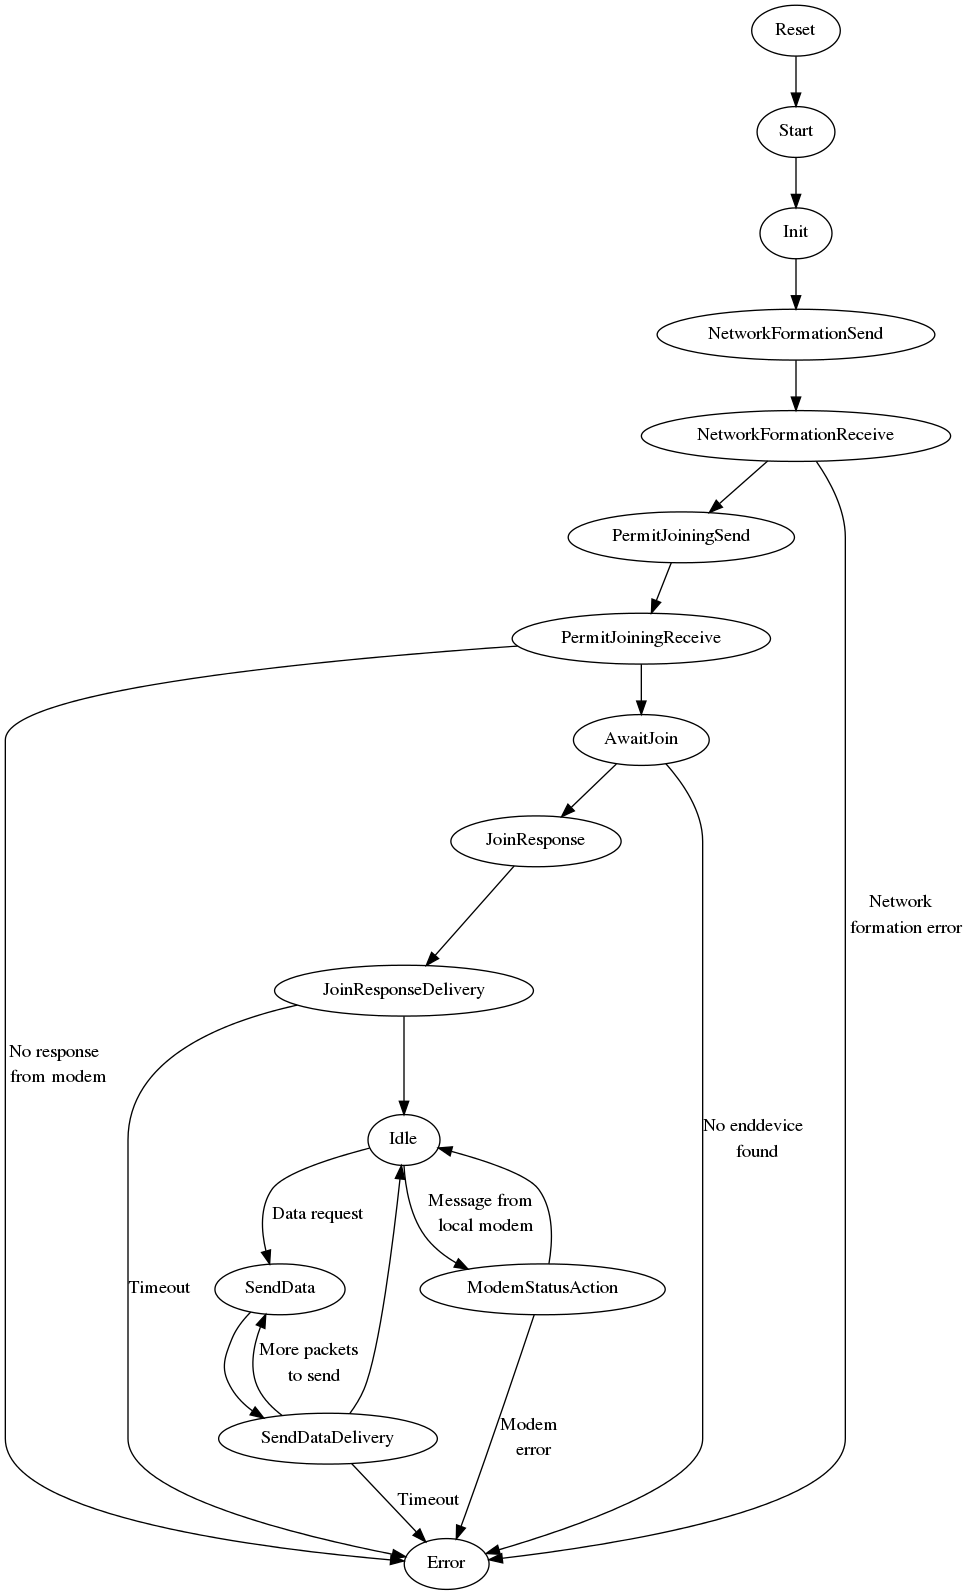
\includegraphics[scale=0.3, angle=0]{basFSM.png}
\end{center}
\caption{Flödesschema över radio i basstation}
\label{fig:radio_bas}
\end{figure}

Radiolänk-delen i implementeringen av basstationen är internt uppbyggd runt en tillståndsmaskin, se figur~\ref{fig:radio_bas} på sida~\pageref{fig:radio_bas}. Syftet med detta är att ge programmeraren kontroll och översikt över exakt vilka kommandon och svar som förväntas, och att programmet endast kan befinna sig i ett av ett antal väldefinierade tillstånd. Basstationen börjar sin livscykel i ett reset-tillstånd, och går vidare till att starta upp coordinator-funktionen och nätverket, sedan lyssna efter anslutande skyltmoduler. Då en skyltmodul anslutit sig går basstationen in i ett passivt lyssningstillstånd. I detta läge väntar basstationen på inkommande statusmeddelanden från det lokala XBee-modemet eller på dataförfrågningar från skylten. Användaren kan även påverka basstationen genom det fysiska gränssnittet under lyssningstillståndet. \\

Då en dataförfrågan mottas, sänder basstationen över den aktuella textdatan via radiolänken och väntar på att skylten ska verifiera överföringen. Då överföringen verifierats återvänder basstationen till sitt passiva lyssningstillstånd. Om basstationen vid något tillfälle avviker från de väldefinierade tillstånden, får ett oväntat och ohanterbart svar eller måste vänta för länge på svar, går den in i ett felläge och signallerar detta till omvärlden. \\

\begin{figure}[H]
\begin{center}
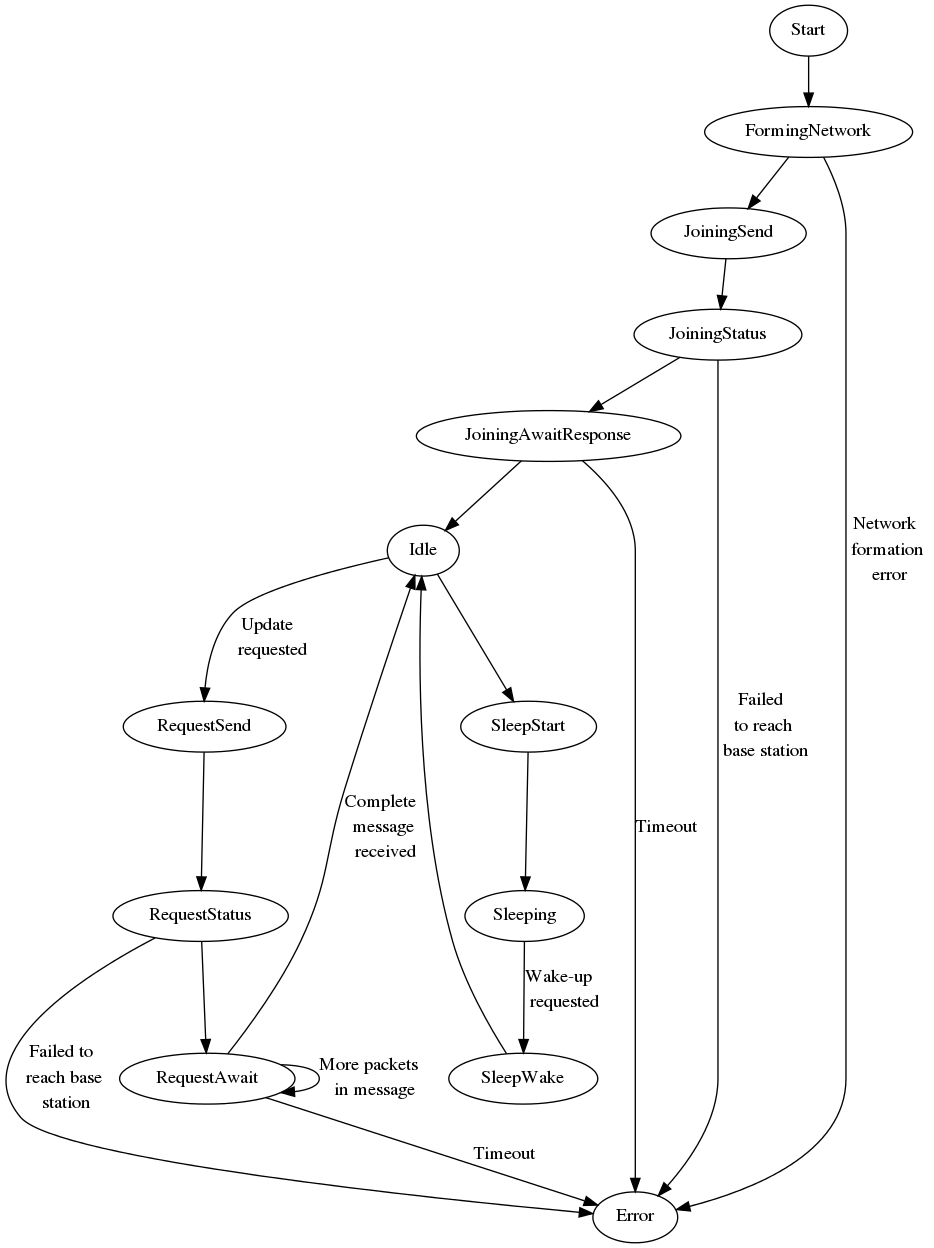
\includegraphics[scale=0.3, angle=0]{skyltFSM.png}
\end{center}
\caption{Flödesschema över radio i skylt}
\label{fig:radio_skylt}
\end{figure}

Skyltmodulens radio är uppbyggd på ett liknande sätt som basstationen, och en beskrivning ges av figur~\ref{fig:radio_skylt} på sida~\pageref{fig:radio_skylt}. Skyltmodulen börjar vid omstart att initiera sin radio, och försöker sedan ansluta sig till en basstation. Sammankopplingen mellan skylt och basstation genomförs genom att skylten skickar en förfrågan om att gå med i nätverket, som sedan identifieras av basstationen. Om förfrågan lyckas sparar basstationen undan skyltmodulens hårdvaruadress för framtida kommunikation och skickar tillbaka ett svarsmeddelande. I det här läget har basstation och skylt anslutit sig till samma nätverk och kan börja kommunicera. Då skylten är i vila är den försatt i ett strömsparläge, och radion är avstängd. Med jämna mellanrum kommer skylten att vakna upp, aktivera sin radiomodul och skicka en dataförfrågan till basstationen. Basstationen svarar med den senaste hämtade textdatan, som skylten sedan tar emot och visar upp på sin display. Detta är det normala operationsläget för skylten. Om skyltens tillståndsmaskin går utanför detta beteende kommer en felhanteringsmetod att anropas.

\subsection{Display}
För att kunna visa upp twittermeddelandena på skyltmodulen krävs det att den har en display. Till detta har vi valt en ChLCD (Cholesteric Liquid Crystal Display) från Kent Displays. Det är en grafisk bistabil LCD som har en upplösning på 240x160 pixlar med en bildyta på 61x41 mm . Pixlarna på kanten runtom bildytan är större än de andra pixlarna för att enkelt kunna göra en dekorativ ram runt innehållet som visas på displayen \hyperref[kent]{(Kent, 2010)}.

Displayen skall kunna visa upp 160 tecken som beskrivits i avsnittet \hyperref[skylt]{(Moduluppdelning - skylt)}, vilket ger utrymme att använda 240 pixlar per tecken. Med exempelvis tecken som är 12 pixlar breda och 20 pixlar höga kan man utnyttja hela displayen och det finns gott om pixlar till att visa upp tydliga tecken. Notera att tomt utrymme mellan tecken ingår i de 240 pixlarna.

Det är viktigt att tecknen är lätta att läsa även på avstånd eftersom typisk användning innebär att man kan vilja se om meddelandet uppdateras genom att kasta en snabb blick när man går förbi skyltmodulen, och den fasta monteringen innebär att det är omöjligt att få skyltmodulen i ögonhöjd för alla som kan tänkas vilja läsa från den.

\subsubsection{Displayens energieffektivitet}
För att maximera skyltens batteritid är viktigt att displayen är energisnål. Eftersom den valda displayen endast kräver ström då den uppdateras passar den bra med resten av skyltmodulen som spenderar större delen av tiden i ett lågenergiläge och inte kräver uppdateringar av displayen.

För att avgöra hur energisnål displayen är jämförs den med LCD-displayer av konventionell typ. Se tabell~\ref{tab:kenttable}. Den alfanumeriska displayen är av en enklare typ som dock klarar av att visa lika många tecken. Den grafiska displayen är av liknande storlek och upplösning som Kent-displayen.

\begin{table}[h]
\centering
    \begin{tabular}{|l|c|c|r|}
    {\bf Modell} & {\bf Statisk} & {\bf Uppdatering} & {\bf Genomsnitt} \\
    Kent & $0$ & $97$ & $0.41$ \\
    Alfanumerisk 160 tecken & $1.75$ & $1.75$ & $1.75$ \\
    Grafisk 240x128 pixlar & $10.9$ & $10.9$ & $10.9$ \\
    \end{tabular}
\caption{Jämförelse av effektförbrukning i ett urval av displayer. [mW]}
\label{tab:kenttable}
\end{table}

Strömförbrukningsvärdena har hämtats från respektive displays datablad \hyperref[lcdalfa]{(DISPLAY Elektronik, 2009)}, \hyperref[lcdgraph]{(DISPLAY Elektronik, 2011)}. Kent-displayens genomsnittsförbrukning togs fram med antagandet att en uppdatering tar 1,27 sekunder, vilket anges som en typisk uppdateringstid vid rumstemperatur i displayens datablad \hyperref[kent]{(Kent Displays Inc., 2010)}. Vi räknar med att uppdatering utförs var 5:e minut, den högsta uppdateringsfrekvensen som uppnås vid normalt användande av skylten.

Trots att den alfanumeriska displayen är av en enklare modell och vi har antagit att displayen uppdateras så ofta som möjligt så kräver Kent-displayen en fjärdedel så mycket energi. Vid normalt användande med färre uppdateringar skulle Kent-displayen kräva ännu mindre energi medan de andra skulle ligga kvar på samma nivå.

Andra displayer baserade på bistabila tekniker var i åtanke under projektet, framförallt de av E-paper typ. Deras långa ledtider och dåliga tillgänglighet ledde dock till att de fick räknas bort.

\subsubsection{Displayens uppbyggnad och användningssätt}
Kent-displayen består utav en ChLCD-panel och en styrenhet. Styrenheten sköter uppdateringen av panelen och innehåller ett 32 kByte stort minne för att lagra data som kan visas på panelen. Displayen styrs genom att kommandon skickas till styrenheten via ett SPI gränssnitt. Ett flertal olika kommandon finns, men till de viktigaste hör att skriva till och läsa från minnet, uppdatera hela eller delar av displayen med data från minnet och att försätta displayen i ett lågenergiläge.

För att visa data på displayen måste först ett kommando utföras som överför datan till minnet, sedan ytterligare ett kommando som faktiskt visar datan på displayen. Datan överförs som minst en byte i taget till minnet i displayen. Då datan skall visas upp på panelen kan man välja att uppdatera 1 till 80 pixelrader eller hela panelen på en gång.

Med uppdateringskommandot anges vilken adress i minnet datan skall börja läsas ifrån. Den mest signifikanta biten på den byte som adressen pekar på utgör den första pixeln på den första raden som skall uppdateras. Nästa bit representerar nästa pixel, nästa byte representerar således 9:e till 16:e pixeln. De första 30 byten utgör hela den första raden. Om fler rader skall uppdateras utgör de följande 30 byten raden under. Detta mönster följs för alla rader som skall uppdateras.

\subsubsection{Hantering av tecken och teckensnitt}

Displayen har inga inbyggda funktioner för att visa upp text, utan Arduinon i skyltmodulen måste översätta texten som skall visas upp på displayen till pixelrepresentation utav texten. Skyltmodulsarduinon har därför ett typsnitt lagrat i programminnet där den kan slå upp tecken och få ut en pixelrepresentation av tecknet. Typsnittet som valdes består av tecken med samma storlek som i exemplet i början av detta delkapitel, 12x20 pixlar. Alla tecken har således samma storlek vilket gör dem lätta att hantera. Det är en modifierad version av linuxsystemfonten, som innehåller alla tecken som skall kunna visas upp på displayen enligt begränsningarna för projektet. För att anpassa typsnittet från 10x18 pixlar till 12x20 pixlar lades tomt utrymme höger och nedanför tecknet till.

Med den första anpassningen av typsnittet hade vissa tecken färgade pixlar ända ut till kanten på utrymmet avsett för tecknet. Om dessa tecken skrevs nära kanten på displayen överlappade tecknet de större rampixlarna och gav ett oönskat utseende. Se figur~\ref{fig:fontA}. Därför gjordes anpassningen om där tecken centrerades på deras teckenområde, vilket gör att de yttersta pixlarna på varje teckens teckenområde aldrig är aktiva. Således undviks problemet med att vissa tecken skrivs på ramen.

\begin{figure}[H]
\begin{center}

\includegraphics[scale=0.5, angle=0]{fontA.png}
\end{center}
\caption{Del av ett A}
\label{fig:fontA}
\end{figure}

Ett exempel från det slutgiltiga typsnittet kan ses i figur~\ref{fig:fontAA}. Varje normalstor pixel på displayen är 0,26 mm bred och hög vilket ger ett teckenområde (hela oranga området) på 3,4 x 5,5 mm. För att sätta detta i perspektiv är tecknen på displayen ungefär lika stora som de i typsnittet {\it Times New Roman} i storleken 16 punkter.

\begin{figure}[H]
\begin{center}

\includegraphics[scale=0.5, angle=0]{fontAA.png}
\end{center}
\caption{Ett litet å}
\label{fig:fontAA}
\end{figure}

Översättningen från tecken till pixlar görs genom att varje rad i texten behandlas var för sig. Pixelrepresentationen av en textrad består av 20 pixelrader, eftersom alla tecken är 20 pixlar höga. Pixelraderna skapas och överförs en och en till displayens minne. En pixelrad byggs upp genom att textraden gås igenom och för varje tecken slås motsvarande pixelrad i tecknet upp för att sedan konkatineras med resterande teckens pixelrader. Om till exempel en textrad består av tecknen AB så kommer första pixelraden att innehålla första raden i tecknet A följt av första raden av teckent B. Nästa pixelrad består av andra pixelraden i A och andra pixelraden i B. Då samtliga 20 pixelrader har skickats iväg till displayens minne påbörjas arbetet med eventuella efterföljande textrader.

\subsection{Övriga uppkopplingar}
Systemet använder en uppsättning handbyggda kretsar för små uppgifter såsom användargränssnitt. Dessa kretsar är relativt simpla och befinner sig i konstruktionens utkant. Detta kapitel beskriver de sådana kretsar som byggts inom ramarna för projektet.

\subsubsection{Avkoppling och kondensatorbank}
XBee-modulerna på basstationen och skylten matas med 5V och 3.3V, från sina respektive arduinoplattformar. För att buffra mot eventuella störningar på matningsspänningen används avkopplingskondensatorer av olika storlek, som rekommenderat i databladet för XBee-modulerna. \\

Skyltens display matas med 3.3V och jord från arduinoplattformen. Mellan display och arduino finns en kondensatorbank inkopplad, med en i sammanhanget stor elektrolytkondensator på 470$\mu$F, och två mindre, snabbare 10$\mu$F-kondensatorer. 

\subsubsection{Knappar och Statusindikatorer}
De knappar som används är enkla tryckknappar med pull-up-motstånd och små kondensatorer. Då en knapp trycks ned kopplas signalen ned till jord. Innan signalen skickas vidare som insignal till målarduinoplattformen skickas den genom en 7414 Schmitt-trigger med inverterarverkan, vilket gör insignalen från knappen aktiv hög. Vidare används LEDs som statusindikatorer, kopplade till digitala utgångar på arduinoplattformarna. Samma princip för tryckknappar och statusindikatorer används på både basstation och skyltmodul.

\subsubsection{Batteri}
Batteriet som driver skylten är ett en-cells Litium-Polymerbatteri på 2000mAh, ger 3.7V och har inbyggt skydd mot överspänning ($>4.25V$), för stort strömuttag och skydd för minimumspänning ($<2.75V$).

\subsubsection{Batterinivåavläsning}
Batterinivån på skyltmodulen avläses genom att en analogingång på skyltens arduinoplattform kopplas till en spänningsdelare. Spänningsdelaren slås till och från via en NMOS-transistor, och microcontrollern läser av spänningen via en A/D-omvandlare.

\subsubsection{Batteriladdning}
Batteriet laddas via en kontakt på basstationen. Det kort som används för att ladda batteriet tar sin matningsspänning och jord från Arduinoplattformen (5V) och reglerar ner spänningen till lämplig nivå för att ladda Litium-Polymer-batteriet. Övriga komponenter på kortet är kondensatorer enligt rekommendationerna för spänningsregulatorn, samt resistanser som fungerar som strömbegränsande för lysdioder. Laddningsstatus visas på en LED.

\subsubsection{Inbyggnadslådor och mekanik}
Delsystemen (skylt och basstation) är inbygga i ABS-plastlådor där hål borrats ut för kontakter, knappar och statusindikatorer. Alla mekaniska delar är byggda för att kunna plockas isär och sättas ihop igen smidigt. M3-skruv har använts genomgående. En kylfläns har lagts till för att kyla spänningsregulatorn på basstationens microcontrollerplattform, då det upptäcktes att den blev varm vid systemdrift med nätadapter.

\section{Systembeskrivning, programlogik}
Med begreppet programlogik avses den del av systemets kod som behandlar problemdomänen. Problemdomänen är en modell av de uppgifter som systemet ska utföra, fri från hänsyn till implementationsdetaljer.\\

Vid uppstart av skylten går den in i en evig loop och skickar var femte minut en förfrågan till basstationen om vilket meddelande som ska visas upp. När ett svar har tagits emot visas meddelandet och dess metadata upp på displayen.\\

Vid uppstart av basstationen läses en konfiguration in för att ställa in vilka meddelanden som ska hämtas in från Twitter och vilken tidszon som datum ska visas i. Om någon av inställningarna är ogiltiga meddelas ett fel.\\

Efter att inställningarna har lästs in går basstationen in i en evig loop och väntar på förfrågningar om meddelanden från skylten. När en förfrågan tas emot så hämtar basstationen in det senaste meddelandet från Twitters API som går igenom användarens filter. Om ett svar tas emot formateras meddelandet och skickas till skylten för att visas upp.

\subsection{Konfigurering av systemet}
En viktig funktion är att kunna konfigurera basstationen med vilket Twitter-konto den ska hämta tweets ifrån, då det inte är speciellt användarvänligt att hårdkoda detta. Användaren av den elektroniska Twitter-skylten ska inte behöva editera i källkoden eftersom det blir onödigt omständigt samt en risk för kompileringsfel. Lösningen blev en konfigurationsfil lagrat på ett SD-kort där användaren kan ange vilket Twitter-konto som skall användas samt en söksträng.
Systemet konfigureras vid uppstart av basstationen genom att läsa av det SD-kort som sitter i basstationens Ethernet Shield. SD-kortet förväntas innehålla en textfil med namnet config.txt. Den första strängen i filen ska innehålla namnet på den Twitter-användare vars tidszon datumet ska visas i. Därefter följer en söksträng med vilken användaren kan specificera vilka tweets som skall visas på skylten med hjälp av bland annat hashtags. Saknas söksträngen hämtas samtliga tweets skrivna från användarens konto. Användandet av söksträngar beskrivs i avdelningen \hyperref[twitterapi]{Twitters API}.


\subsubsection{Inläsning}
För att läsa från SD-kortet användes Arduinos standard bibliotek för SD-kort som i sin tur använder biblioteket sdfatlib \hyperref[arduino]{(Arduino, 2012f)}. Konfigurationsfilens namn måste följa 8.3 konventionen eftersom sdfatlib begränsas av det \hyperref[arduino]{(Arduino, 2012f)}. Detta innebär att filnamnet får högst ha ett åtta tecken långt namn följt av en filändelse på maximalt tre tecken \hyperref[microsoft]{(Microsoft, 2012)}.\\

I konfigurationsfilen ska varje inställning separeras med mellanslag, tab eller nyradstecken. Först kommer användarnamnet därefter söksträngen. När filen har öppnats allokeras ett minnesutrymme som är lika många bytes som filen är stor. Sedan läses hela filen in i minnet med undantag av blanktecken före och efter användarnamnet. När inläsningen är klar är det känt hur många signifikanta tecken som är inlästa. Om det är färre inlästa tecken än antalet i filen så allokeras ett nytt minnesutrymme som endast har plats för adekvata tecken. Minnesutrymme som tidigare bestod av vittecken kan på så vis frigöras. Slutligen exponeras inställningarna för systemet genom metoder som returnerar dessa.

\subsection{Förnyelse av IP-adress via DHCP}
För att kommunicera över internet krävs det att basstationen har en IP-adress \hyperref[cisco]{(Cisco Systems, 2003)}. Tilldelningen kommer att ske med hjälp av nätverkets DHCP-server, som har en samling med lediga adresser. För att DHCP-servern inte ska få slut på adresser så är det brukligt att en lånetid sätts, det vill sig hur länge enheten kan vara säker på att ha den givna adressen. Arduinos Ethernet-bibliotek (v1.0) har inte implementerat stöd för att uppdatera lånetiden av IP-adressen, vilket kan leda till att kontakten med internet förloras.\\

Då DHCP initeras försöker basstationen att få IP-adress av DHCP-servern genom att skicka DHCP Discover meddelanden \hyperref[cisco]{(Cisco Systems, 2003)}. Om den inte får svar inom en minut så slutar den försöka. Om det däremot kommer ett erbjudande om IP-address från servern så svarar basstationen på erbjudandet och accepterar adressen. Basstationen har då IP-adressen under den period som servern har bestämt.    

\subsubsection{Implementation}
I enighet med DHCP ska förnyelseförsök av IP-adress ske vid halva lånetiden, T1, och vid sju åttondelar av lånetiden, T2, om det inte lyckades första gången. Första förfrågan sker endast till DHCP-servern som lånar ut IP-adressen till klienten, medan den andra förfrågningen går ut till alla på nätverket genom broadcast. En förfrågan ska gå till så att klienten skickar sitt meddelande med längre och längre intervall till dess att den får svar eller att 60 sekunder har passerat \hyperref[droms]{(Droms, 1997)}. Får klienten svar uppdateras dess lånetid och eventuella IP-adressändringar genomförs.\\

Hantering av lånetidsuppdatering kan implementeras med:

	\begin{enumerate}
	\item Timer som ger avbrott
    	\item En funktion som anropas för tidavläsning
	\end{enumerate}
	
Fördelen med alternativ 1 är att uppdateringen sker automatiskt när timern genererar ett avbrott. Nackdelarna är att timern i basstationens mikrocontroller slår över alltför ofta relativt till hur långa lånetider på IP-adresser det oftast är, vilket kräver en räknare för att utöka tidsrymden. Dessutom skulle det behövas totalt tre timerar för T1, T2 och lånetiden.\\

I alternativ 2 används millis, en funktion som finns i Arduinomiljön, den räknar antalet millisekunder modulo $2^{32}$ sedan enheten startades och kan läsas av samtidigt som tiden fortskrider. Anrop till millis används för att jämföra aktuell tid med tiden då IP-adressen blev lånad för att avgöra om lånetiden behöver uppdateras. Funktionaliteten implementeras i en funktion som ska anropas med jämna mellanrum. Fördelen med alternativ 2 är att med enkla jämförelser kan det avgöras när förnyelse ska ske. Nackdelen är att tiden måste läsas av varje varv i programloopen, att det inte kan styras exakt när kontrollen av lånetiden görs och det kan hända att IP-adressen används efter lånetiden löpt ut.\\

Den slutliga lösningen blev alternativ 2, eftersom att programloopen ska köras ofta och att millis redan är implementerad. Vidare valdes alternativ 1 bort eftersom att ATmega2560 endast har fyra 16-bitars timerar vilka kan behövas i andra delar av programmet.\\

Implementationen bryter mot DHCP specifikationen på några punkter:

	\begin{itemize}
	\item Om lånetiden är mindre än åtta minuter blir det problem om förnyelse misslyckas eftersom en förfrågan kan ta upp till 60 sekunder. Under den tiden kan lånetiden redan passerat och     basstationen använder IP-adressen felaktigt.
    	\item Då millis slår över går det inte att kontrollera om lånetiden är slut. I det fallet görs ett försök att låna om IP-adressen omedelbart även om inte T1 har passerats.
	\end{itemize}	

Eftersom att basstationen kommer vara ansluten till ett trådbundet nätverk kommer första punkten inte vara något problem, eftersom att den minsta låntiden i praktiken är 15 minuter \hyperref[wen]{(Windows Enterprise Networking, 2007)}. Andra punkten är endast en rekommendation som bryts och då det blev alltför besvärligt att hantera millis överslag, som sker en gång ungefär vart 50:e dygn. Den effektivaste lösningen är således att begära förnyelse av IP-adressen vid överslag på millis.
	
\subsection{HTTP}
För att hämta information från Twitter använder sig systemet av HTTP, som är det kommunikationsprotokoll som ligger till grund för webben. HTTP används för att skicka och ta emot resurser utifrån klient/server-modellen: En klient skickar en förfrågan till en server, som skickar tillbaka ett svar. En resurs är ett abstrakt begrepp som i IETF:s specifikation definieras som något med en identitet. De resurser som systemet efterfrågar från Twitter är användaruppgifter samt meddelanden och deras metadata. \\

HTTP är textbaserat och kommunicerar över TCP. Både klienter och servrar använder sig av valfria portnummer, men för servrar är det vanligtvis port 80.

\subsubsection{Förfrågan}

En HTTP-förfrågan består av fem delar:
	
	\begin{enumerate}
    	\item En metod, som anger hur resursen ska behandlas.
    	\item En URL, som anger vilken resurs som ska behandlas.
    	\item Ett versionsnummer, som anger vilken version av HTTP som ska användas. (Systemet använder version 1.1.)
    	\item En lista med headers, som anger diverse alternativ och metadata.
    	\item En meddelandekropp, som anger eventuell data som ska skickas till servern.
	\end{enumerate}

HTTP har stöd för ett antal olika metoder, däribland GET, POST, PUT och DELETE. I systemet används enbart förfrågningar med GET-metoden, som begär att resursens innehåll skickas tillbaka som svar.
	
\subsubsection{Svar}
	
Ett HTTP-svar liknar en HTTP-förfrågan och består av fyra delar:

	\begin{enumerate}
    	\item Ett versionsnummer.
    	\item En statuskod följt av en statusbeskrivning.
    	\item En lista med headers.
    	\item En meddelandekropp.
    	\end{enumerate}

\subsection{JSON}

JSON är ett textbaserat format för överföring av data. Det är ett av två format som används i svaren på förfrågningar till Twitters API; det andra är XML. Eftersom JSON har en enklare datamodell och mindre verbos syntax är den att föredra i sammanhang där minnesutrymmet och processorkraften är begränsad. Av denna anledning tar systemet emot data från Twitters API i JSON-format.

	\begin{itemize}
	\item Nummer
    	\item Sträng
    	\item Booleanvärde
    	\item Fält
    	\item Objekt
    	\item Null
	\end{itemize}

Av dessa datatyper är fält och objekt sammansatta: De innehåller andra värden av valfri typ. I fält är dessa värden indexerade med heltal i stigande ordning från noll. I objekt är dessa värden indexerade med strängar som är unika inom det objektet (nycklar). \\

En JSON-fil består av antingen ett objekt eller ett fält, som i sin tur kan innehålla ytterligare värden enligt reglerna för respektive datatyp. \\

Den förväntade statusen i svaret på en GET-förfrågan är {\it 200 OK}, som innebär att resursen har bifogats i svarets meddelandekropp som avsett. \\

\subsubsection{Avläsning och intolkning}
Vanligtvis tolkas JSON genom att läsa av hela filen och lagra den i en datastruktur i minnet som tillåter godtycklig navigering. Problemet med parsingen när den ska utföras på en Arduinoplattform är att mängden RAM-minne är begränsad till 8 kilobyte. Risken är således stor att ett fullständigt inläst JSON-svar från Twitters API tillsammans med övrig programdata tar slut på systemets minne. \\

För att lösa detta problem används en händelsebaserade strömparser. Till skillnad från en konventionell parser lagrar en händelsebaserad strömparser inte JSON-datan i minnet. Istället signalerar parsern händelser varje gång den påträffar ett värde medan den läser av JSON-filen. Dessa händelser hanteras sedan av en uppsättning olika funktioner som anropas av parsern genom funktionspekare. Detta tillvägagångssätt innebär att minnesåtgången är minimal eftersom enbart det värde som precis har lästs av behöver sparas i minnet. \\

Den parser som används i systemet heter Yajl. Den signalerar en händelse varje gång som den påträffar något av följande:

	\begin{itemize}
    	\item Nullvärde
    	\item Booleanvärde
    	\item Heltal
    	\item Decimaltal
    	\item Nummervärde
    	\item Sträng
    	\item Början på objekt
    	\item Objektnyckel
    	\item Slut på objekt
    	\item Början på fält
    	\item Slut på fält
	\end{itemize}
	
Dessa motsvarar en händelse för varje datatyp med följande undantag:

	\begin{itemize}
	\item Händelsen för nummervärden anropas för både heltal och decimaltal.
    	\item Ett värde av en komposit datatyp ger upphov till flera händelser: en för dess början, en för dess slut samt en för varje nyckel som ingår i det (om det är ett objekt). Varje värde som ingår i objektet eller fältet ger dessutom upphov till händelser som vanligt utifrån dess datatyp.
    	\end{itemize}
    	
Ett av problemen med en händelsebaserad parser som Yajl är att dess sekventiella inläsning gör det svårare att deklarativt hämta in data från JSON-filen genom att exempelvis ange en sökväg. Yajl har visserligen inbyggt stöd för att hämta in data genom att ange en sökväg ({\it simplified tree interface}), men detta kräver att hela JSON-filen läses in i minnet på samma gång och fungerar enbart med värden inuti objekt, inte värden inuti fält. Av denna anledning behöver inhämtningen av data implementeras på imperativ väg genom de funktionspekare som anropas vid olika händelser.

\subsubsection{Algoritm}

Den inhämtning av data som används i vårt system är baserad på en väldigt enkel princip: En lista med objektnycklar matas in och för varje objektnyckel sparas det första värde som förknippas med den objektnyckeln, oavsett var i JSON-filen objektnyckeln befinner sig.

Avläsningen av JSON-filen inleds med följande algoritm:

	\begin{enumerate}
    	\item En tabell definieras med objektnycklar och variabler, där varje objektnyckel förknippas med en variabel.
    	\item Parsern läser av JSON-filen och signalerar en händelse så fort någon av objektnycklarna i listan påträffas.
	\end{enumerate}

Så fort en händelse signaleras utförs denna algoritm:
	
	\begin{enumerate}
    	\item Nästa värde som läses in av parsern sparas i den variabel som förknippas med den nyligen inlästa objektnyckeln.
    	\item Den nyligen inlästa objektnyckeln och variabeln som den är förknippad med tas bort från tabellen.
	\end{enumerate}

Algoritmen skulle kunna implementeras så generellt som den är beskriven ovan, men eftersom systemet hämtar in så pass få olika värden (tre stycken) är den istället implementerad genom individuell hantering av varje enskilt fall; slutresultatet är samma.

Denna metod har två begränsningar:

	\begin{enumerate}
    	\item Endast ett enda värde kan läsas in för varje objektnyckel som anges, så det är omöjligt att läsa in separata värden som befinner sig i olika delar av JSON-filen men har samma objektnyckel.
    	\item Endast det första värdet som förknippas med en angiven objektnyckel kan läsas in, så det är omöjligt att komma åt värden vars objektnycklar har förekommit tidigare i JSON-filen.
	\end{enumerate}

Dessa begränsningar är dock inga problem i systemet eftersom inga av de objektnycklar som behöver läsas in förekommer mer än en gång i något av de svar som tas emot från Twitters API. Eftersom Twitters API dessutom är versionsangivet bör risken vara minimal att beteendet förändras i framtiden, och om en godtycklig förändring mot förmodan sker så skulle också alla andra algoritmer för avläsning potentiellt kunna misslyckas.

\subsection{Twitters API}
Twitters API består av ett antal URL:er som kan efterfrågas med HTTP för att komma åt stora delar av Twitters innehåll. Systemet använder sig av detta API för att komma åt två olika delar av Twitters innehåll: användaruppgifter och meddelanden. \\

\subsubsection{Användaruppgifter}

Varje meddelande ska visas på skylten tillsammans med datum och tid, men samtliga meddelanden som skickas från Twitters API har datum och tid angivet i UTC (GMT-tidszonen). För att visa rätt datum och tid måste systemet komma åt användarens tidszon. Denna finns tillgänglig i form av en UTC-offset i användarens offentliga uppgifter. Dessa uppgifter skickas som svar på förfrågningar till följande URL, där namn är namnet på den användare vars meddelanden ska visas: \url{api.twitter.com/1/users/show.json?screen_name=namn}. Användarnamnet erhålls av systemet genom konfigurationsfilen.

Svaret innehåller ett objekt med flera olika värden. Användarens UTC-offset har nyckeln {\it $utc_offset$} och representeras som ett heltal med tecken där värdet anger skillnaden i sekunder mellan användarens tidszon och UTC. Denna offset hämtas in en enda gång när systemet startar och lagras i programmets minne för att senare användas vid infogandet av metadata i användarens meddelanden.

Värt att notera är att denna UTC-offset inte inkluderar eventuell tidsskillnad på grund av sommartid. Eftersom basstationen inte själv innehåller någon klocka så hanterar systemet inte heller denna tidsskillnad, utan det krävs att användaren själv ändrar inställningarna på sitt Twitter-konto för att rätt tid ska visas på skylten. En möjlig lösning på problemet är att låta användaren själv ange sin tidszon i konfigurationsfilen, men detta valdes bort då det skulle leda till en mer komplicerad implementation och ett mer komplicerat användargränssnitt.

\subsubsection{Meddelanden}
Den söksträng som användaren har angivit i konfigurationsfilen används för att hämta de meddelanden som ska visas på skylten. De meddelanden som matchar söksträngen skickas som svar på förfågningar till följande URL, där där söksträng är den angivna söksträngen: \url{http://search.twitter.com/search.json?q=söksträng&result_type=recent&rpp=1}. De parametrar utöver söksträngen som ingår i URL:en har följande verkan:

	\begin{itemize}
    	\item {\it $result_type=recent$} sorterar de matchande meddelandena efter publiceringsdatum i fallande ordning.
    	\item {\it $rpp=1$} begränsar antalet resultat till ett. {\it $rpp$} står för {\it $return per page$} \hyperref[twitter]{(Twitter, 2012b)}.
	\end{itemize}

Söksträngar som ingår i förfrågningar till Twitters sök-API använder samma syntax som den vanliga sökfunktionen på Twitters hemsida. Denna syntax finns dokumenterad på Twitters hemsida \hyperref[twitter]{(Twitter, 2012a)}.

\subsubsection{Begränsningar}
Twitters API och systemets användning av det lyder under följande begränsningar:
	
	\begin{itemize}
     	\item Meddelanden som är äldre än en vecka kan inte hämtas in (Twitter, 2012). Twitters sök-API kan bara användas för att hitta meddelanden som är “ungefär en vecka” gamla (“omkring 6-9 dagar” i en annan del av dokumentationen). Detta är inget problem så länge basstationen är aktiverad, men så fort den stängs av och sätts på igen kommer den enbart att ha tillgång till meddelanden från den senaste veckan. Om det senaste meddelandet är äldre kommer den felaktigt att rapportera till skylten att inga meddelanden finns tillgängliga. Om skylten sedan stängs av (exempelvis för att laddas) kommer den vid uppstart inte att ha tillgång till det meddelande som den visade upp före avstängning.
    	\item Vissa meddelanden kan saknas helt i sökresultaten. Eftersom Twitters sök-API “fokuserar på relevans, inte fullständighet” (Twitter, 2012). Vilka meddelanden som saknas är inte tydligt dokumenterat, och det är också ytterst svårt att testa. I värsta fall kan denna begränsning leda till utelämnade meddelanden vid godtyckliga tillfällen.
    	\item Systemet förlitar sig på en sökoperator som inte är dokumenterad. För att utelämna retweets från API-svaren använder sig systemet av sökoperatorn “+exclude:retweets”. I samtliga tester har den fungerat som avsett men i värsta fall kan dess beteende ändras i framtiden. Om operatorn helt skulle försvinna skulle det innebära att systemet också tar emot retweets, som kan innehålla fler än 140 tecken. För att säkerställa att detta scenario aldrig leder till några problem läses endast de 140 första tecknen av samtliga meddelanden in. Detta leder till att retweets som visas på skylten kan få viss text utelämnad men aldrig krascha systemet.
    	\item Meddelanden kan inte hämtas in i realtid. Eftersom Twitters REST-baserade API som svar på varje förfrågan enbart skickar den data som är aktuell vid samma tidpunkt måste klienten regelbundet skicka förfrågningar för att få den senaste datan. Twitter erbjuder också ett strömbaserat API som kontinuerligt skickar data i realtid (Twitter, 2012), men detta kräver autentisering vilket gör klientens implementation och användargränssnitt mer komplicerat.
    	\item Meddelanden kan hämtas in högst 150 gånger per timme (Twitter, 2012). Twitters API begränsar antalet förfrågningar per IP-adress till 150 per timme. Detta innebär att systemet maximalt kan skicka förfrågningar ungefär två gånger per minut. Eftersom systemet frågar efter nya meddelanden mindre ofta än detta är denna begränsning inget problem.
    	\end{itemize}
    	
\subsection{Formatering}
Efter att ett meddelande har tagits emot från Twitters API men innan det visas upp på skylten behöver det formateras. Formateringen innefattar fyra områden:
	\begin{enumerate}
    	\item Omkodning: Att hantera tecken som displayen inte kan hantera genom att ersätta dem mot andra.
    	\item Normalisering: Att radera överflödiga blanksteg i början av, i slutet av och inuti meddelandet.
    	\item Justering: Att fördela orden i meddelandet över bildskärmens rader så att så få ord som möjligt behöver brytas upp över två rader.
    	\item Metadata: Att lägga till metadata till meddelandet i form av ett numeriskt publiceringsdatum.
	\end{enumerate}

Resultatet av formateringen är en displaysträng som kan skickas från basstationen till skylten för att visa upp meddelandet och dess metadata.

\subsubsection{Omkodning}
De meddelanden som tas emot från Twitters API innehåller Unicode-tecken kodade i UTF-8. Eftersom displayen inte har stöd för UTF-8 behöver tecknen kodas om till den uppsättning som stöds. Displayen har stöd för ASCII-tecken samt bokstäverna Å, Ä och Ö, och är således lämplig för både engelska och svenska meddelanden.\\

Eftersom Arduino inte har inbyggt stöd för konvertering till och från UTF-8 så omkodar basstationen meddelandena från Twitters API enligt följande regler:
	\begin{itemize}
    	\item Samtliga ASCII-tecken samt Å, Ä och Ö kodas om från UTF-8 till den representation som de behöver på displayen.
    	\item Övriga tecken ersätts med tilde-tecken ($\sim$).
    	\item Varje UTF-8-tecken som består av flera bytes ersätts med ett enda tilde-tecken, inte ett för varje byte som de upptar.
	\end{itemize}

\subsubsection{Algoritm, omkodning}
UTF-8 är en teckenkodning som tillåter varierande antal bytes för att representera enstaka tecken. En fördel med UTF-8 gentemot många andra teckenkodningar är att UTF-8 även är ASCII-kompatibel, vilket innebär att alla tecken som är giltiga ASCII-tecken också är giltiga UTF-8-tecken. Det är dessutom något som gör algoritmen för att koda om UTF-8-meddelanden till skyltens teckenkodning markant enklare. \\

Konverteringen består av två huvudkomponenter: gruppering av bytes till tecken, och uppslagning av tecken i en teckentabell för att representera ett tecken på skylten i passande kodning. Denna tabell tillåter uppslagning av ett godtyckligt antal tecken, och de tecken som inte har en översättning får således översättas med ett ersättningstecken. \\

Givet en början med textmarkören i strängens början konverteras strängen till önskad teckenkodning på följande sätt.
	
	\begin{enumerate}
    	\item Skapa en tom sträng med plats för lika många tecken som originalsträngen.
    	\item Sök genom strängen byte för byte.
    		\begin{enumerate}
        	\item Om den byte som är under nuvarande markör är ett 7-bitars ASCII-tecken görs en uppslagning i översättningstabellen och det konverterade tecknet läggs till i resultatsträngen. Markören flyttas därefter ett steg framåt.
        	\item Om den byte som är under nuvarande markör har sin åttonde bit satt är tecknet ett multibyte-tecken. Räkna antalet aktiva bitar bland de fyra högre bitarna av nuvarande byte, och flytta markören lika många gånger framåt i strängen. Detta är så många bytes som tecknet under markören bestod av. Uppslagning görs av denna sekvens av bytes i översättningstabellen och läggs till i resultatsträngen.
        	\end{enumerate}
    	\item Om hela strängen har behandlats, avsluta och returnera resultatsträngen. I annat fall återgå till punkt två.
	\end{enumerate}
	
\subsubsection{Normalisering}
För att kunna formatera meddelandet så enkelt och konsekvent som möjligt är det önskvärt att normalisera det så att det har samma struktur som alla andra meddelanden. I detta fall innebär det behandling av meddelandets blanksteg. När meddelandet ska justeras och visas upp blir logiken enklare om vi kan utgå från att varje ord skiljs åt med ett och endast ett mellanslag. På en abstrakt nivå vill vi kunna behandla varje meddelande som en lista av ord där blanktecken (whitespace) inte behöver tas i åtanke. \\

En sådan radering av blanktecken innebär att en användare inte själv kan formatera sina meddelanden genom att infoga extra utrymme i form av blanktecken. Detta är dock konsekvent med Twitters beteende i webbläsaren, där upprepade blanktecken alltid slås samman (collapse) till ett enda blanksteg. \\

Ett meddelande med blanktecken precis i början och i slutet av texten kan publiceras till Twitter, men det är enbart blanktecken inuti texten som returneras av Twitters API. Detta innebär att radering av såna blanktecken inte behöver ingå i algoritmen för normalisering.

\subsubsection{Algoritm, normalisering}
Utgå från att strängen består av en mängd tecken, som alla kan kategoriseras att vara whitespace (blanksteg, nyrad, tab, etc) eller en del av ett ord. För att veta vad som ska returneras gås strängen igenom två gånger: en gång för att räkna ord, och en gång för att extrahera ord.
	\begin{enumerate}
    	\item Sätt nuvarande status till WHITESPACE, och ordräknaren till noll.
    	\item Traversera strängen tecken för tecken.
    		\begin{enumerate}
        	\item Om vår nuvarande status är WHITESPACE.
        		\begin{enumerate}
            		\item Om det tecken som är under markören är en whitespace, gör ingenting.
            		\item Om det tecken som är under markören inte är en whitespace, öka ordräknaren och sätt nuvarande status till WORD.
            		\end{enumerate}
        	\item Om vår nuvarande status är WORD.
        		\begin{enumerate}
            		\item Om det tecken som är under markören är en whitespace, sätt nuvarande status till WHITESPACE.
            		\item Om det tecken som är under markören inte är en whitespace, gör ingenting.
            		\end{enumerate}
            	\end{enumerate}
    	\item Allokera utrymme för returvärdet så att det rymmer det antal strängar som ordräknaren står på. Sätt nuvarande status till WHITESPACE.
    	\item Traversera strängen tecken för tecken.
        Flytta markören till första whitespace.
        Flytta markören till första icke-whitespace.
        Skapa en ny sträng av alla tecken från markören som inte är whitespace. Lägg strängen på första lediga plats i minnet för vårt returvärde.
	\end{enumerate}
	
\subsubsection{Justering}
Systemet använder sig av två olika sätt att justera ett ord som överskrider längden på en rad:

	\begin{enumerate}
    	\item Nedflyttning: Att flytta ned hela ordet till början av nästa rad.
    	\item Avstavning: Att infoga ett bindestreck i ordet och låta första halvan stanna på samma rad medan andra halvan flyttas ned till nästa rad.
	\end{enumerate}

Nedflyttning leder i allmänhet till bra läslighet men kräver mer utrymme än avstavning, i synnerhet när väldigt långa ord flyttas ned. \\

Avstavning leder till ett bättre utnyttjande av displayen men är svårare att implementera, inte minst för att avstavningsregler är olika beroende på vilket språk som meddelandet är skrivet på. Olika approximationer kan göras men ett bra resultat kan endast uppnås med hjälp av bibliotek för språkbehandling. Eftersom sådana kräver betydande utrymme för diverse språkdatabaser kan de inte användas i detta sammanhang. \\
    
Även utan algoritmer för korrekt avstavning kvarstår möjligheten att låta ett ord gå ut till kanten av en rad, infoga ett bindestreck och flytta ned resten av ordet till nästa rad. Systemet avstavar ord på detta sätt. \\

Bedömningen gjordes dock att en sådan {\it naiv} avstavning inte är nämnvärt bättre än att låta ordet brytas upp över två rader utan något bindestreck. Den avstavning som används i systemet utelämnar bindestreck på detta sätt.

\subsubsection{Algoritm, justering}
Den algoritm som vi tog fram för justering är en relativt simpel girig algoritm: Den flyttar ned ord så långt det går och bryter ord över två rader (utan bindestreck) så fort en nedflyttning skulle orsaka platsbrist. Algoritmen tar som argument en lista med ord. \\

För att snabbare kunna testa olika lösningar implementerades algoritmen först som en prototyp i skriptspråket JavaScript.
	\begin{enumerate}
    	\item För varje ord i listan:
    		\begin{enumerate}
        	\item Om ordet får plats på nuvarande rad
        		\begin{enumerate}
        		\item placera ordet på nuvarande rad.
        		\end{enumerate}
        	\item Annars: 
        		\begin{enumerate}
        		\item Beräkna det minsta utrymmet som krävs för att placera de kvarvarande orden med början på nästa rad. 
        		\item Om utrymmet räcker till:
        			\begin{enumerate}
        			\item Placera ordet på nästa rad och fortsätt justeringen därifrån.
        			\end{enumerate}
            		\item Annars (om ordet måste brytas upp över två rader):
            			\begin{enumerate}
                		\item Dela upp ordet i två nya ord: det första så långt som antalet oanvända tecken kvar på raden, det andra bildat av de återstående tecknen.
                		\item Placera det första ordet på nuvarande rad.
                		\item Infoga det andra ordet på nuvarande plats i listan.
                		\end{enumerate}
                	\end{enumerate}
    		\end{enumerate}
    	\end{enumerate}

\subsubsection{Resultat}
Efter att vi hade färdigställt vår första algoritm så övervägde vi att ta fram en mer avancerad algoritm som testar flera olika sätt att justera texten och väljer det bästa, enligt någon definition. Den definition som vi kom fram till var att låta så få korta ord som möjligt brytas över två rader, eftersom korta ord generellt är svårare att läsa än långa ord när de bryts över två rader. Vi beslöt oss dock först för att testa vår första algoritm på faktiska meddelanden från Twitter, för att se hur den fungerar i praktiken.\\

För att genomföra testet hämtade vi in 100 huvudsakligen svenska meddelanden från Twitters API, körde algoritmen på dem och granskade resultatet för hand. Vi kom fram till att vår första algoritm fungerade förvånansvärt bra på dessa godtyckligt utvalda meddelanden. I de flesta av meddelandena kunde samtliga ord flyttas ned istället för att brytas över två rader, vilket ledde till bra läslighet. Vi tror att detta beror på två anledningar:

	\begin{enumerate}
    	\item Eftersom teckengränsen på ett meddelande är 140 tecken så kommer de flesta meddelanden att hamna under det. I och med att ett genomsnittligt ord på Twitter är omkring 6 tecken långt (inklusive föregående mellanslag) så räcker det med att ett eller två ord ska utelämnas av platsbrist för att ett avsevärt utrymme ska sparas in till justering.
    	\item Eftersom vår display har plats för 160 tecken så finns det plats för 20 tecken utöver meddelandets text. 14 av dessa är reserverade åt den datumstämpel som visas efter meddelandet, men de 6 ytterligare tecknen ger extra utrymme för justering.
    \end{enumerate}

Faktum är att praktiskt taget de enda ord i vårt test som behövde brytas över flera rader var URL:er, som lider av samma problem i nästan alla andra medier. I och med detta positiva resultat bestämde vi oss för att använda vår första algoritm i det färdiga systemet.

\subsection{Metadata}
Eftersom displayen har rum för 160 tecken finns det möjlighet att visa mer text än enbart ett meddelande, som högst är 140 tecken långt. Under projektets planeringsfas diskuterades vilken eventuell metadata som skulle visas. Främst diskuterades publiceringsdatum och användarnamn. \\

Publiceringsdatum är önskvärt att visa på displayen eftersom det ger meddelandet ett sammanhang. Många av de meddelanden som sätts upp på dörrskyltar handlar om tillfällig frånvaro, och då är det ofta viktigt för läsarna att veta när meddelandet publicerades. Användarnamn ger också ett sammanhang, men eftersom en dörrskylt redan är fysiskt monterad på användarens kontorsdörr blir informationen vanligtvis överflödig. Vi bestämde oss således för att enbart ta med meddelandets publiceringsdatum som metadata.\\

Datumet visas på formatet {\it dd/mm tt:ss}, där uttrycken syftar på följande information i meddelandets publiceringsdatum:

	\begin{itemize}
    	\item dd: Dagen på månaden, utan inledande nolla (1-31).
    	\item mm: Månadens ordningsnummer, utan inledande nolla (1-12).
    	\item tt: Timmen på dygnet, med inledande nolla (00-23).
    	\item ss: Minuten på timmen, med inledande nolla (00-59).
    	\end{itemize}
    	
Datumet visas i det nedre högra hörnet av displayen och föregås av ett bindestreck följt av ett mellanslag ({\it - dd/mm tt:ss}).\\

En komplikation som uppstår när metadata ska infogas i displayens nedre högra hörn är att algoritmen för avstavning potentiellt kan ha förbrukat detta utrymme genom att flytta ned ord, som i följande exempel med ett 124 tecken långt meddelande. \\

Meddelande:\\

a bbbbbbbbbbbbbbbbbbbbbbbbbbbbbbbbbbbbbbbb cccccccccccccccccccccccccccccccccccccccc dddddddddddddddddddddddddddddddddddddddd

\begin{table}[h]
\centering
	\begin{tabular}{l|}
	a \\
	bbbbbbbbbbbbbbbbbbbbbbbbbbbbbbbbbbbbbbbb \\
	cccccccccccccccccccccccccccccccccccccccc \\
	dddddddddddddddddddddddddddddddddddddddd \\
	\end{tabular}
\caption{Meddelandet efter avstavning och högermarginaljustering}
\label{tab:msgexample}
\end{table}

I exemplet har ordet {\it bbb...} flyttats ned istället för att avstavas eftersom detta lämnar kvar tillräckligt med utrymme för resten av meddelandet. Problemet är att utrymmet i det nedre högra hörnet nu är förbrukat, vilket gör det omöjligt att infoga ett datum. Detta går att lösa genom att justera algoritmen för justering, men detta gör den mer komplicerad och kräver att den har kunskap om hur den justerade strängen ska användas, vilket ökar antalet beroenden mellan funktioner. \\

Istället löses detta problem genom att en 13 tecken lång platshållarsträng infogas i slutet på den lista av ord som ska justeras. Eftersom denna platshållare är lika lång som den metadata som ska infogas i meddelandet (ett datum samt det bindestreck och mellanslag som föregår det) kommer algoritmen för avstavning att garantera att det alltid finns plats över för att infoga metadatan. Infogandet av den faktiska metadatan består sedan av två steg: att ersätta platshållarsträngen med metadatan samt att infoga nyrader och blanksteg så att metadatan visas i displayens nedre högra hörn. \\

Den platshållarsträng som används är {\it 0123456789abc}. Vilken sträng som helst skulle kunna användas så länge den består av 13 tecken och inte innehåller några mellanslag, men den aktuella strängen har en fördel: inga tecken förekommer två gånger. Detta används när metadatan ska placeras på rätt plats i meddelandet, då platshållarsträngens början identifieras genom att söka efter den första nollan från meddelandets slut. 

\subsubsection{Algoritm, metadata}
Datumet läggs till på meddelandet efter att det har justerats. Eftersom det alltid ska visas det nedre högra hörnet av displayen kräver detta viss logik för att implementera, då längden på meddelandet och antalet nyrader i det är okänt.
	\begin{enumerate}
    	\item Räkna antalet nyrader i strängen.
    	\item Infoga nyrader tills det finns tre nyrader i strängen.
    	\item Räkna antalet tecken som föregår platshållaren på den sista raden.
    	\item Infoga blanksteg före platshållaren tills den sista raden är 40 tecken lång.	
    	\item Ersätt platshållaren med metadatan.
    	\end{enumerate}
    	
\section{Resultat}

\subsection{Resultatsammanställning, mätdata och produktegenskaper}

\subsubsection{Funktionalitet}

{\large \it \colorbox{yellow}{TODO: skriva kort om det slutgiltiga systemets funktioner}}

\subsubsection{Energieffektivitet}
För att mäta energieffektivteten har ett antal mätningar, beräkningar och uppskattningar gjorts. Strömförbrukningen för varje delmodul har så långt det gått uppmätts i isolation, och som en del av det kompletta systemet, för att kunna peka ut systemets flaskhalsar. Mätningarna har gjorts vid matningsspänning på 3.7V (från batteriet), som regleras ned till 3.3V för systemet. Alla mätningar har skett vid vanlig rumstemperatur och i övrigt under normala kontorsförhållanden.

\begin{table}[h]
\centering
	\begin{tabular}{|l|r|}
	Arduino Pro 3.3V (aktivt läge) & {$11.4 mA$}\\
	Arduino Pro 3.3V (strömsparläge) & {$16 {\mu}A$}\\
	Spänningsregulator (idle) & {$1 mA$}\\
	{\it Då Arduinoplattformen är aktiv, gäller även:} & { }\\	
	Radiotransceiver (avlyssning/mottagning) & {$51 mA$}\\
	Radiotransceiver (sändning) & {$45 mA$}\\
	Display (uppdatering) & {$40 mA$}\\
	Display (aktiv) &  {$0 mA$}\\
	Batteriavläsning (inaktiv) & {$obetydlig$}\\
	Batteriavläsning (aktiv) & {$4 {\mu}A$}\\
	Per aktiv LED & {$2 mA$}\\
	Per aktiverad knapp & {$30 {\mu}A$}\\
	\end{tabular}
\caption{Strömförbrukning, enskilda moduler}
\label{tab:currentdrawtable}
\end{table}

Den slutsats som direkt kan dras är att spänningsregulatorn är den största källan till energiförlust, utslaget över en längre period. Detta beror på att resistiva förluster (i form av värme) fås i regulatorn då spänningen regleras ned till $3.3V$ för systemet. Resultatet blir även att regulatorn blir varm. Lite efterforskning ger dock resultatet att den regulator som används är väl anpassad för systemet och batteriet. Det finns dyrare regulatorer som skulle kunna ge bättre energieffektivitet. \\

Med uppdateringsintervall på $5$ minuter och uppdateringstid på $10$ sekunder för en komplett uppdatering av skylten (med display och radiokommunikation) ger detta en batteritid på strax över $690$ timmar $(\approx 29 dagar)$ pessimistiskt räknat. I denna beräkning har antagits att radion är aktiv hela tiden och maximalt antal omsändningar görs. Beräkningen tar dock inte hänsyn till förluster i ledningar, regulatorn för XBee-modulen eller temperaturförändringar. Av dessa uppskattas dock endast XBee-modulens spänningsregulator ha en mätbar inverkan, och även den bör vara mycket liten. \\

Uppskattningsvis och optimistiskt räknat, fås en maximal batteritid på strax under $1200$ timmar $(\approx 50 dagar)$. En noggrannare och rimligare uppskattning av driftstiden för systemet ligger runt $800-860$ timmar $(\approx 32-36 dagar)$ på ett fulladdat batteri, inräknat alla mätbara faktorer och under antagandet att användande av skylten sker enligt det normala användarscenario som beskrivs tidigare i rapporten. Som väntat är det alltså spänningsregulatorerna som är de största källorna till förluster. Med perfekta spänningsregulatorer beräknas systemet kunna ha en batteritid på uppmot $100$ dagar. \\

Arduinoplattformen använder sig av en linjär spänningsregulator, vilket innebär att överbliven effekt går förlorad som värme. Den överblivna effekten kommer av differensen i spänning mellan vad som fås ut av batteriet och systemets driftsspänning. Ett alternativ skulle vara att använda en så kallad switchande spänningsregulator. Dessa kräver dock mer avancerade uppkopplingar och är dyrare \hyperref[dimension]{(Dimension Engineering, 2012)}. \\

\begin{figure}[H]
\begin{center}
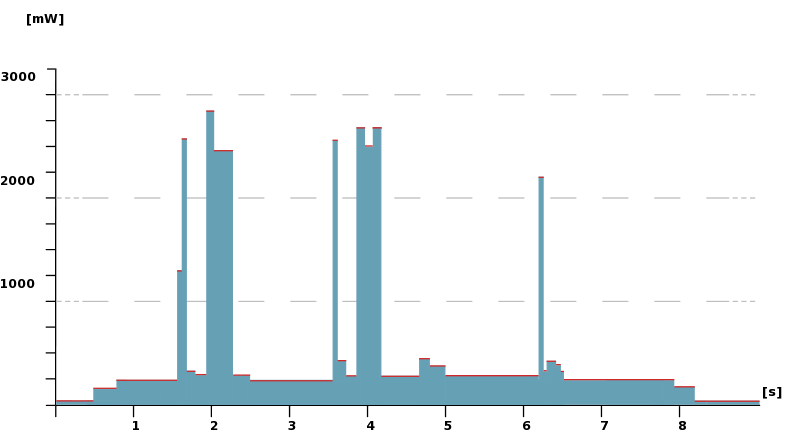
\includegraphics[scale=0.70, angle=0]{effekt.png}
\end{center}
\caption{Effektanalys för skylt}
\label{fig:effectgraph}
\end{figure}

Systemet är försatt i strömsparläge den allra största delen av driftstiden. Aktiv tid uppgår till maximalt $3\%$, typiskt $1\%$ av tiden, beroende mestadels på radiokommunikationen. Under sömnperioden är effektförbrukningen relativt liten, men under en längre period. Som motsats är uppdateringsperioden kort, flera effektförbrukningsspikar uppträder under uppdateringen. Dessa kommer av radiokommunikation (sändning och mottagning), samt uppdatering av display. Displayen uppdateras mycket snabbt, och sändning av data går också idealt snabbt, dock med risk för omsändning vid misslyckande. Mottagning av och avlyssning efter data på radiolänken är den aktivitet som bidrar mest till energiförbrukningen under uppdateringscykeln. Figur~\ref{fig:effectgraph} visar effektförbrukning i hela systemet under en uppdateringscykel, där två datapaket tas emot från basstationen. De spikar som noteras kommer från radion, först sändning, sedan mottagning, samt från display.

\begin{figure}[H]
\begin{center}
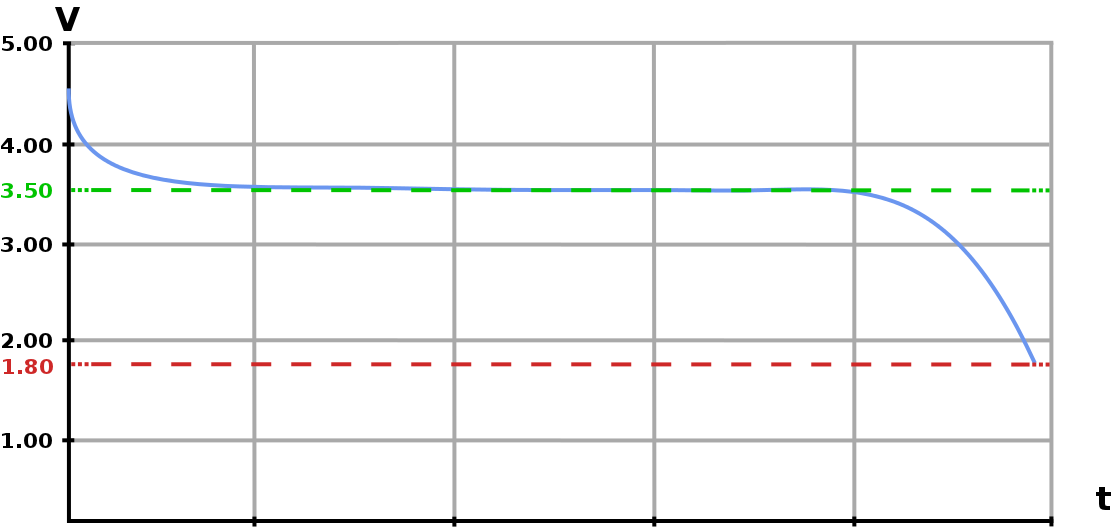
\includegraphics[scale=0.35, angle=0]{battery.png}
\end{center}
\caption{Urladdningsförlopp för LiPo-batteri}
\label{fig:batterygraph}
\end{figure}

Batteriet som valdes visade sig vara ett mycket bra val, då det ger en lång batteritid, men fortfarande är litet och smidigt nog att bygga in i produkten. Eftersom det rör sig om ett LiPo-batteri så har dock den avläsningsmetod som används i projektet visat sig vara otillräcklig. LiPo-batterier har en relativt konstant spännings-tid-kurva, undantaget relativt skarpa förändringar i början och slutet av urladdningscykeln. \\

Batteriavläsningen tar för närvarande endast hänsyn till den spänning som fås ut från batteriet, vilket inte fungerar som en bra indikator för laddningsstatus. Figur~\ref{fig:batterygraph} visar att spänningen som fås från batteriet hålls relativt konstant under urladdningscykeln, fram till en skarp nedåtsväng mot slutet. En alternativ lösning för batteristatusavläsning togs fram, där systemet konstant håller reda på strömmen som dras från batteriet, och utför en integration av strömmen. Med kompletterande information om batteriets initiala laddning kan därefter kvarvarande laddning räknas ut. Vidare fås detaljerad information om hur batteriet används, som kan användas till att räkna fram en uppskattning av återstående batteritid. \\

Denna lösning är dock inte implementerad i systemet, då det skulle innebära mycket extra beräkningskraft som går åt till att beräkna batteritid, samt en del extra hårdvara. Bland annat skulle en avläsningsbar strömprob behöva kopplas till microcontrollern, samt att externa minneskretsar skulle behöva läggas till för att spara datan relaterat till batterihanteringen. Inom projektet togs snabbt beslutet att detta skulle vara mycket onödigt, på grund av extra kostnader och platsbrist, både fysiskt i enheten och i form av I/O-pinnar på microcontrollern. Vidare skulle det bidra relativt lite till användarupplevelsen. Med nuvarande lösning ger systemet en varning om att batterinivån är låg då spänningen från batteriet börjar sjunka. Då vet samtidigt användaren om att det verkligen är dags att ladda batteriet, då batterinivåvarningen kommer relativt sent i urladdningscykeln. Användaren informeras om den låga batterinivån via en status-LED på skylten. \\

\subsubsection{Radiolänk och nätverk}
Radiolänken har testats i kontorsmiljö (Instutitionen för Data- och informationsteknik på Chalmers), och fungerar bra. Ihopparning av modulerna går relativt snabbt (ca 5 sekunder), och inga konflikter med närliggande nätverk märks av. Vid systemstart kan basstationen ta upp till en minut på sig att ansluta sig till nätverksuppkopplingen via DHCP, men oftast går det snabbare. \\

Radiokommunikationen har testats även över längre avstånd inomhus, och verkar fungera bra upp till ungefär två våningar upp eller ned i ett vanligt kontorshus. Även cirka 40-50 meter i sidoled. Detta ger en radie runt basstationen som skylten kan operera inom. Operationsområdet för skylten begränsas av väggar, annan störande elektronisk utrustning och andra fysiska hinder. Sammantaget bedöms radiokommunikationen väl uppfylla de krav på räckvidd och samexistensförmåga med andra nätverk som finns i en vanlig kontorsmiljö, och därmed uppfyller radionätverket även den specifikation som ställdes upp i början av projektet. Test har inte utförts utomhus, då det är utanför skyltens tänkta användningsområde. \\

Robustheten i radiokommunikationen är relativt god. Vid längre avstånd gör systemet fler omsändningar av data över radiolänken, på grund av paketförluster. Dessa bidrar till längre uppdateringstider för skylten, men är acceptabla. Små avstånd (upp till 10 meter) ger mycket goda förhållanden mellan misslyckade och framgångsrika paketsändningar. Vid enstaka tillfällen händer det att många paket i följd tappas, vilket får som resultat att systemet går in i ett felhanteringsläge. Detta sker dock sällan, och endast vid långa avstånd med fysiska hinder för radiokommunikationen.

\subsubsection{Fysiska dimensioner}
\begin{table}[h]
\centering
	\begin{tabular}{|l|c|c|c|}
	Basstation & 150 & 80 & 50 \\
	Skylt & 150 & 80 & 20 \\
	\end{tabular}
\caption{Fysiska dimensioner}
\label{tab:dimensiontable}
\end{table}

Systemets något stora och klumpiga fysiska dimensioner beror på att inbyggnadslådorna och elektroniken är hanterad för hand och med vanliga labb- och hemverkstadsverktyg. Skylten är smidig nog att hänga upp på en dörr, och basstationen är relativt lätt att ställa undan obemärkt på ett vanligt kontor. Ingen av enheterna gör ljud eller har någon nämnvärd värmeutveckling som begränsar placeringsmöjligheterna. Även vikten hos enheterna är låg. På detta sätt kan de fysiska dimensionerna anses uppfylla kravspecifikationen, men vid serieproduktion skulle inbyggnadslådorna och elektroniken behöva göras mindre och smidigare.

\section{Diskussion och slutsatser}

\subsection{Utvärdering av projektupplägg}

{\large \it \colorbox{yellow}{TODO: diskuteras på Torsdagens (10/5) gruppmöte}}

\subsection{Sidospår och problem under projektet}

\subsubsection{Operationslägen för XBee}
Ett tidigt sidospår inom projektet var designvalet att basera radiolänken på XBee:s AT-läge. AT-läget är ett simpelt kommunikationsläge som kan ses som en trådlös ersättning av en serielänk, och har till skillnad från API-läget inte stöd för några avancerade protokollfunktioner som omsändning och paketinkapsling. Efter att ha arbetat med AT-läget och byggt upp en fungerande radiolänk, togs valet att gå över till API-läget på grund av den robustare kommunikationen och bättre kontrollen över radiolänkens status. Vidare behövde meddelanden delas upp i flera paket som dessutom behövde samordnas mellan varandra, vilket är olämpligt att implementera med XBee:s AT-läge.

\subsubsection{Kanalsökning för radio}
Under ett tidigt stadie i utvecklingen fick gruppen problem med XBee:s förmåga att söka genom radiomiljön efter energinivåer i alla de olika frekvenskanalerna inom operationsområdet. Problemet bestod i att det tog för lång tid att söka genom alla kanaler, och det var inte hållbart att ta den första tillgängliga. Problemet löstes genom att radion konfigurerades för att använda fasta inställningar, och klarar nu av att ställa upp en fungerande radiolänk på kort tid. 

\subsubsection{Kondensatorbank för display}
Basstationen drivs med 12V från nätspänning via en transformator, och behöver inga extra kondensatorer. Skylten däremot drivs endast av ett en-cells LiPo-batteri. Detta ger problem vid systemstart då skyltens display startas upp och ska uppdateras. \\

Problemet upptäcktes då gruppen skulle föra över skylten från en testuppkoppling på breadboard till den hårdvara som ingår i den slutgiltiga prototypen. Systemet startade om sig upprepade gånger, och displayen blinkade utan att skriva ut någonting. Efter mycket felsökning och försök till problemisolering föll misstanken på avkopplingskondensatorerna, som antogs vara för små. Ytterligare experiment genomfördes, och slutsatsen blev att systemet fungerade endast om det kopplades upp med matningsspänning via en breadboard. Mer felsökning och tester följde, och resultatet var förvånande: ledningarna i breadboarden fungerade som kapacitanser, vilket gjorde att testuppkopplingen på breadbord, men inte den slutgiltiga prototypen, klarade av att uppdatera displayen. \\

Lösningen på problemet blev att lägga till extra avkopplingskondensatorer mellan spänning och jord för hela systemet, samt en extra stor kondensatorbank mellan matningsspänning och jord till displayen. Flera olika kapacitanser testades innan det avgjordes att en stor elektrolytkondensator (470$\mu$F) behövdes. Till detta lades två mindre (10$\mu$F) och snabbare kapacitanser för att ta bort högfrekventa störningar och hjälpa till att snabbare ladda upp elektrolytkondensatorn. \\

Dessa kondensatorer behövs för att hantera den strömspik som displayen ger upphov till då den startas och uppdateras. Strömspiken kommer av displayens strömförsörjningssystem och dess kondensatorer som skall laddas upp. Utan kondensatorbanken faller spänningen i systemet till cirka halva matningsspänningen vid displayuppdatering. Upp- och urladdningsförloppen i kondensatorbanken går mycket snabbare än displayens uppdateringstid, och utgör därmed inget problem tidsmässigt.

\subsubsection{Problem med Arduinos bootloader}
I projektets slutfas slutade programmeringen av Arduino Mega:n (basstationen) att fungera. Elektrisk felsökning genomfördes på hårdvaran, men utan att något problem hittades. Efterforskningar på Arduinos forum gjordes, och det visade sig vara ett fel i konstruktionen av Arduinons bootloader, som gör att om vissa tecken eller sekvenser finns i den källkod som laddas upp, kan bootloadern gå in i ett felaktigt läge och fastna. Bootloadern är den del av Arduinos källkod som behövs för att starta igång den användarprogrammerade koden. \\

Gruppen övervägde flera alternativ, bland annat att försöka bygga basstationen runt en annan typ av Arduino, men detta valdes bort på grund av den minnesbrist det skulle medföra. Efter en del arbete lyckades gruppen lägga in en ny bootloader på Arduino Mega:n, och arbetet kunde fortsätta. Det vanliga sättet att lägga in bootloaders på Arduinokort, via Arduinos utvecklingsmiljö, fungerade inte. Istället fick de så kallade Fuse-bits sättas manuellt, vissa hårdvaruregister skrivas över, och en hex-fil föras över med hjälp av en extern programmeringskrets.

\subsubsection{Minnesbrist vid parsing}
Projektet stötte på ett problem när JSON-data ifrån Twitter skulle parsas. Då JSON strängen innehöll escape-tecken så fungerade inte parsningen med parser biblioteket YAJL och basstationen startade helt plötsligt om. Det misstänktes det att åtgången av RAM-minnet var för stort och att detta orsakade omstarten. Efter undersökning av parserns källkod upptäcktes det att en buffer allokerades när den stötte på ett escape-tecken. Hur mycket minne som parsern försökte allokera styrdes av ett standard värde som var inställt på 2 kB, vilket kan jämföras med basstationens totala RAM-minne på 8 kB. Standard värdet ansågs var för högt inställt och när det minskades flöt parsningen på som förväntat.

\subsubsection{E-Paper}
Originaltanken var att basera skylten runt en E-paper-display. Detta ändrades först under projektets slutfas, då E-paper fanns vara för dyrt och svårtillgängligt med bland annat controllerkort och leveranstider på produkterna. Istället valdes en ChLCD, en annan energieffektiv displayteknik. Såsom marknaden ser ut i dagsläget väntas inte E-paper eller ChLCD kunna konkurrera på den vanliga displaymarknaden under de närmaste åren, på grund av avsaknad av bra färgdisplayer och långa uppdateringstider \hyperref[epapercentral]{(Epaper Central, 2012)}.

\subsection{Jämförelser med liknande projekt}
En enkel google-sökning ger en handfull projekt som involverar Twitter och Arduino. Det främsta exemplet på ett liknande projekt är även det som gav grundtanken till detta projekt, Erico Guizzo:s artikel Send a Tweet to Your Office Door i IEEE Spectrum, Juni 2011 \hyperref[spectrum]{(Guizzo, IEEE Spectrum, 2011)}. Guizzo:s projekt skiljer sig dock på en del viktiga punkter, det är inte trådlöst eller har energieffektivitetsfokus (bland annat används en mindre energieffektiv display), samt att slutprodukten är relativt otymplig. Guizzo:s projekt är även tekniskt enklare och har mindre inbyggd robusthet och felhantering. \\

Ett annat projekt, Arduino LCD Twitter Display, implementerar liknande funktioner, men har liknande nackdelar som Guizzo:s projekt, i form av energiineffektivt, icke-trådlöst och otympligt. Här behöver Arduino-enheten även direkt koppling till en PC \hyperref[instructables]{(Instructables, 2011)}. \\

Inget annat projekt erbjuder en twitteransluten, trådlös dörrskylt med energieffektiv display och radio, eller lång batteritid. Vidare finns inget annat projekt som erbjuder samma robusta kommunikationslänk eller användarvänlighet. Hummingbird kräver inte heller någon extern PC för att koppla upp sig mot internet, utan använder egen nätadapter för matningsspänning, och går att koppla direkt till en router via vanlig Ethernet. \\

\subsection{Expansionsmöjligheter}
En expansionsmöjlighet till projektet, som diskuterades tidigt under planeringsfasen, är att lägga till möjligheten för flera skyltar att ansluta sig till samma basstation. Vidare finns vidareutvecklingspotential för radion och sättet på vilket den anpassar sig till närliggande nätverk. \\

Andra tänkbara vidareutvecklingar är tillägg av möjlighet för användaren att komma åt och konfigurera basstationer via ett webb-interface, eller att kontrollera hela nätverk av basstation-skyltpar via sitt lokala nätverk eller via internet. \\

Rent produktionstekniskt skulle systemet kunna anpassas för serieproduktion med relativ lätthet, givet industriell utvecklingsutrustning. Med för ändamålet specialutvecklade mönsterkort och ytmonterade komponenter skulle de fysiska dimensionerna på enheterna kunna krympas avsevärt. Vidare skulle kostnaderna per enhet sjunka dramatiskt vid serieproduktion. Användarvänligheten hos systemet skulle kunna förbättras genom att göra det lättare att komma åt SD-kortet och att byta och ladda skyltens batteri. 

\pagebreak

\clearpage
\phantomsection
\addcontentsline{toc}{section}{Referenser}
\bibliographystyle{apalike}
\begin{thebibliography}{9}

\label{atmel}
\bibitem{atmel}
   Atmel, \\
   \begin{list}{[\alph{qcounter}]}{\usecounter{qcounter}}
   \item \emph{ATMega328P}.
   \url{http://www.atmel.com/devices/ATMEGA328.aspx} (2012-01-24)
   \item \emph{ATMega2560}.
   \url{http://www.atmel.com/devices/ATMEGA2560.aspx} (2012-01-24)
   \item \emph{ATMega328P Datablad}.
   \url{http://www.atmel.com/Images/doc8271.pdf} (2012-02-15)
   \end{list}
   2008-2012.

\label{arduino}
\bibitem{arduino}
   Arduino,\\
   \begin{list}{[\alph{qcounter}]}{\usecounter{qcounter}}
   \item{\emph{Arduino}. \url{http://www.arduino.cc/} (2012-01-19)}
   \item{\emph{Arduino Pro}. \url{http://arduino.cc/it/Main/ArduinoBoardPro} (2012-01-19)}
   \item{\emph{Arduino Mega}. \url{http://arduino.cc/it/Main/ArduinoBoardMega} (2012-01-19)}
   \item{\emph{XBee Shield} \url{http://arduino.cc/it/Main/ArduinoXbeeShield} (2012-01-24)}
   \item{\emph{Ethernet Shield} \url{http://arduino.cc/en/Main/ArduinoEthernetShield} (2012-01-19)}
   \item{\emph{Arduino SD} \url{http://arduino.cc/en/Reference/SD} (2012-04-14)}
   \end{list}
   2009-2012.

\label{cisco}
\bibitem{cisco}
    Cisco Systems,
    \emph{CCNA 3 and 4 Companion Guide (Cisco Networking Academy Program), ss. 14, 391-392.}.
    Cisco Press, Indianapolis, USA,
    Upplaga 3,
    2003.

\label{dell}
\bibitem{dell}
    Dell,
    \emph{Wireless vs. Wired},
    \url{http://www.dell.com/content/topics/topic.aspx/global/learn/network/plan_vs?c=us&l=en&cs=19},
    2012. (2012-04-27)

\label{digi}
\bibitem{digi}
    Digi,\\
    \begin{list}{[\alph{qcounter}]}{\usecounter{qcounter}}
    \item\emph{XBee Series 1},
    \url{http://ftp1.digi.com/support/documentation/90000976_J.pdf} (2012-01-24)
    \item \emph{XCTU},
    \url{http://www.digi.com/support/productdetail?pid=3352&osvid=57&type=cabling} (2012-02-23)
    \item \emph{Choosing an XBee Antenna},
    \url{Choosing an XBee Antenna http://www.digi.com/technology/rf-tips/2007/08} (2012-01-27),
    \end{list}
    2012

\label{dimension}
\bibitem{dimension}
    Dimension Engineering,
    \emph{A beginner’s guide to switching regulators},
    \url{http://www.dimensionengineering.com/info/switching-regulators},
    2012. (2012-04-29)

\label{lcdalfa}
\bibitem{lcdalfa}
    DISPLAY Elektronik GmbH.,
    \emph{LCD MODULE DEM 240128D FGH-PW. DISPLAY Elektronik GmbH.},
    \url{http://www.display-elektronik.de/DEM240128D_FGH-PW.pdf},
    2009. (2012-05-07).

\label{lcdgraph}
\bibitem{lcdgraph}
    DISPLAY Elektronik GmbH.,
    \emph{LCD MODULE DEM 40491 SYH-LY. DISPLAY Elektronik GmbH.},
    \url{http://www.display-elektronik.de/DEM40491SYH-LY.PDF},
    2011. (2012-05-07).

\label{eetimes}
\bibitem{eetimes}
    Drew Gislason, 
    EE Times,
    \emph{ZigBee Applications},
    \url{ http://www.eetimes.com/design/embedded-internet-design/4201087/ZigBee-applications--Part-1-Sending-and-receiving-data/},
    2010. (2012-02-25)

\label{embedded}
\bibitem{embedded}
    Embedded Computing,
    \emph{Smart energy apps making the move to ZigBee: Q\&A with Oyvind Strom, PhD, Senior Director of Wireless Microcontrollers, Atmel Corporation},
    \url{http://embedded-computing.com/smart-microcontrollers-atmel-corporation-2#ixzz1Xs7COh4m},
    2011. (2012-02-05)

\label{epapercentral}
\bibitem{epapercentral}
    Epaper Central,
    \url{http://www.epapercentral.com/},
    2012. (2012-03-29)

\label{spectrum}
\bibitem{spectrum}
    Erico Guizzo, 
    IEEE Spectrum,
    \emph{Send a tweet to your office door},
    \url{http://spectrum.ieee.org/geek-life/hands-on/send-a-tweet-to-your-office-door},
    2011. (2012-01-17)

\label{instructables}
\bibitem{instructables}
    Instructables,
    \emph{Arduino LCD Twitter Display},
    \url{http://www.instructables.com/id/Arduino-LCD-Twitter-display/},
    2011. (2012-01-17)

\label{droms}
\bibitem{droms}
    Droms, R.,
    \emph{Dynamic Host Configuration Protocol. The Internet Engineering Task Force.},
    \url{http://www.ietf.org/rfc/rfc2131.txt},
    1997. (2012-04-05)

\label{kent}
\bibitem{kent}
    Kent Displays Inc,
    \begin{list}{[\alph{qcounter}]}{\usecounter{qcounter}}
    \item \emph{Kent Displays},
    \url{http://www.kentdisplays.com/},
    2012. (2012-04-05) \\
    \item \emph{1/8 VGA Cholesteric Display Module with SPITM-Compatible Interface. Kent Displays | Resources.},
    \url{http://www.kentdisplays.com/services/resources/datasheets/25075h_240x160_SPI_datasheet.pdf},
    \end{list}
     2012. (2012-03-31)

\label{microsoft}
\bibitem{microsoft}
    Microsoft,
    \emph{Naming, Files, Paths, and Namespace},
    \url{http://msdn.microsoft.com/en-us/library/aa365247.aspx},
    2012. (2012-XX-XX)

\label{mingu}
\bibitem{mingu}
    M. Gu.,
    \emph{The World of Liquid Crystal Displays - Cholesteric Liquid Crystal},
    \url{http://www.personal.kent.edu/~mgu/LCD/chlc.htm},
    2006. (2012-04-19)

\label{lavrentovich}
\bibitem{lavrentovich}
    O.D. Lavrentovich, M.Gu, et al.,
    \emph{Electro-Optical Effects in Liquid Crystals with Dielectric Dispersion},
    Proc. SPIE, 
    Vol. 7050, 70500S,
    2008.

\label{processing}
\bibitem{processing}
    Processing,
    \emph{Processing},
    \url{http://www.processing.org/},
    2012. (2012-03-30)

\label{sensornetworks}
\bibitem{sensornetworks}
    Sensor Networks,
    \emph{Triple Security in ZigBee: Link, Network and Application layer Encryptions},
    \url{http://sensor-networks.org/index.php?page=1010510536},
    2010. (2012-02-05)

\label{techon}
\bibitem{techon}
    TechOn,
    \emph{Entire Surface of Handset Becomes LCD Display},
    \url{http://techon.nikkeibp.co.jp/english/NEWS_EN/20090609/171529/},
    2009. (2012-03-30)

\label{national}
\bibitem{national}
    The National
    \emph{Facebook and Twitter key to Arab uprisings: report},
    \url{http://www.thenational.ae/news/uae-news/facebook-and-twitter-key-to-arab-spring-uprisings-report},
    2011. (8/5/2012)

\label{twitter}
\bibitem{twitter}
    Twitter,
    \begin{list}{[\alph{qcounter}]}{\usecounter{qcounter}}
    \item \emph{How to Use Advanced Twitter Search}, \url{https://support.twitter.com/articles/71577}, (8/5/2012)
    \item \emph{Twitter turns six}, \url{http://blog.twitter.com/2012/03/twitter-turns-six.html}, (8/5/2012)
    \item \emph{REST API Resource}, \url{https://dev.twitter.com/docs/api}, (8/5/2012)
    \item \emph{Using the Twitter Search API}, \url{https://dev.twitter.com/docs/using-search}, (8/5/2012)
    \item \emph{Streaming API}, \url{https://dev.twitter.com/docs/streaming-api}, (8/5/2012)
    \item \emph{Rate Limiting}, \url{https://dev.twitter.com/docs/rate-limiting}, (8/5/2012)
    \end{list}
    2012

\label{wen}
\bibitem{wen}
    Windows Enterprise Networking,
    \emph{Configuring lease time.},
    Microsoft Windows DHCP Team Blog,
    \url{http://blogs.technet.com/b/teamdhcp/archive/2007/02/07/configuring-lease-time.aspx},
    2007. (2012-0X-XX)

\label{wiring}
\bibitem{wiring}
    Wiring,
    \emph{Wiring},
    \url{http://wiring.org.co/},
    2012. (2012-03-30)

\label{wiznet}
\bibitem{wiznet}
    WIZnet Co., Ltd.,
    \emph{W5100.  WIZnet.},
    \url{http://www.wiznet.co.kr/Sub_Modules/en/product/Product_Detail.asp?cate1=5&cate2=7&cate3=26&pid=1011},
    2012. (2012-04-04)

\label{xbeearduino}
\bibitem{xbeearduino}
xbee-arduino,
\emph{xbee-arduino},
\url{http://code.google.com/p/xbee-arduino/},
2011. (2012-02-01)

\label{zigbee}
\bibitem{zigbee}
    ZigBee Alliance,
    \emph{ZigBee},
    \url{http://www.zigbee.org/Specifications/ZigBee/Overview.aspx},
    2012. (2012-01-24)

\end{thebibliography}

\appendix
\renewcommand{\appendixpagename}{Appendix}
\appendixpage
\renewcommand{\appendixtocname}{Appendix}

\addappheadtotoc

\section{Blockschema, basstation}

\begin{figure}[H]
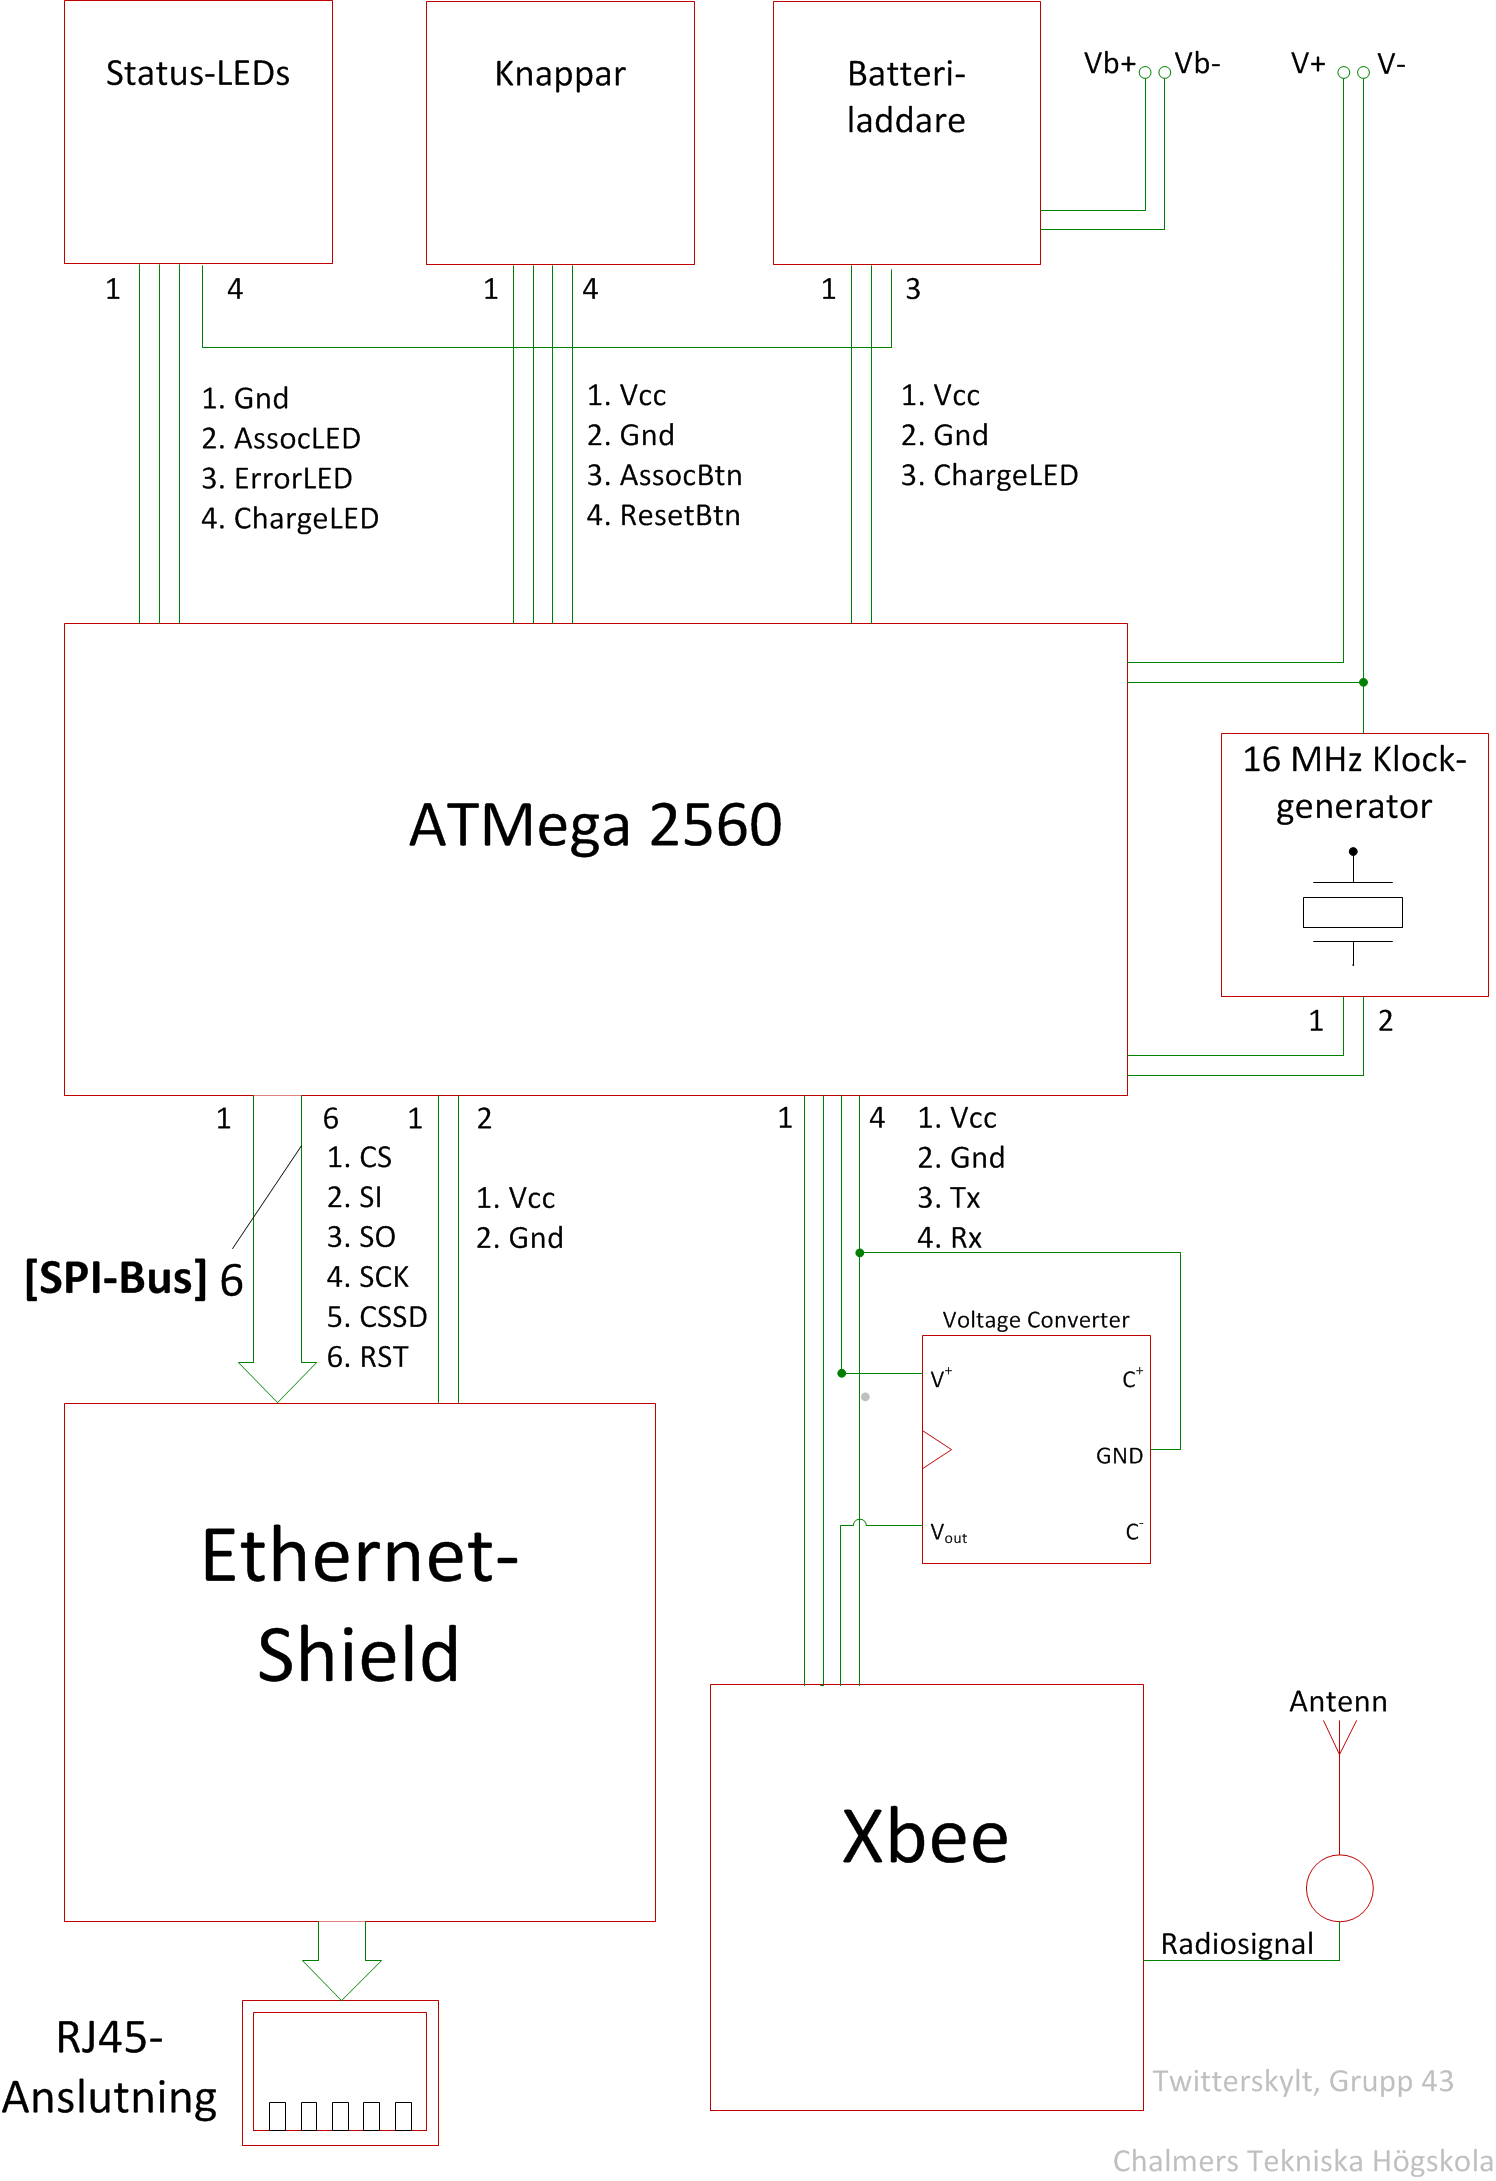
\includegraphics[scale=0.6, angle=0]{block_bas.png}
\label{fig:block_bas}
\caption{Blockschema, basstation}
\end{figure}
\pagebreak

\section{Blockschema, skylt}

\begin{figure}[H]
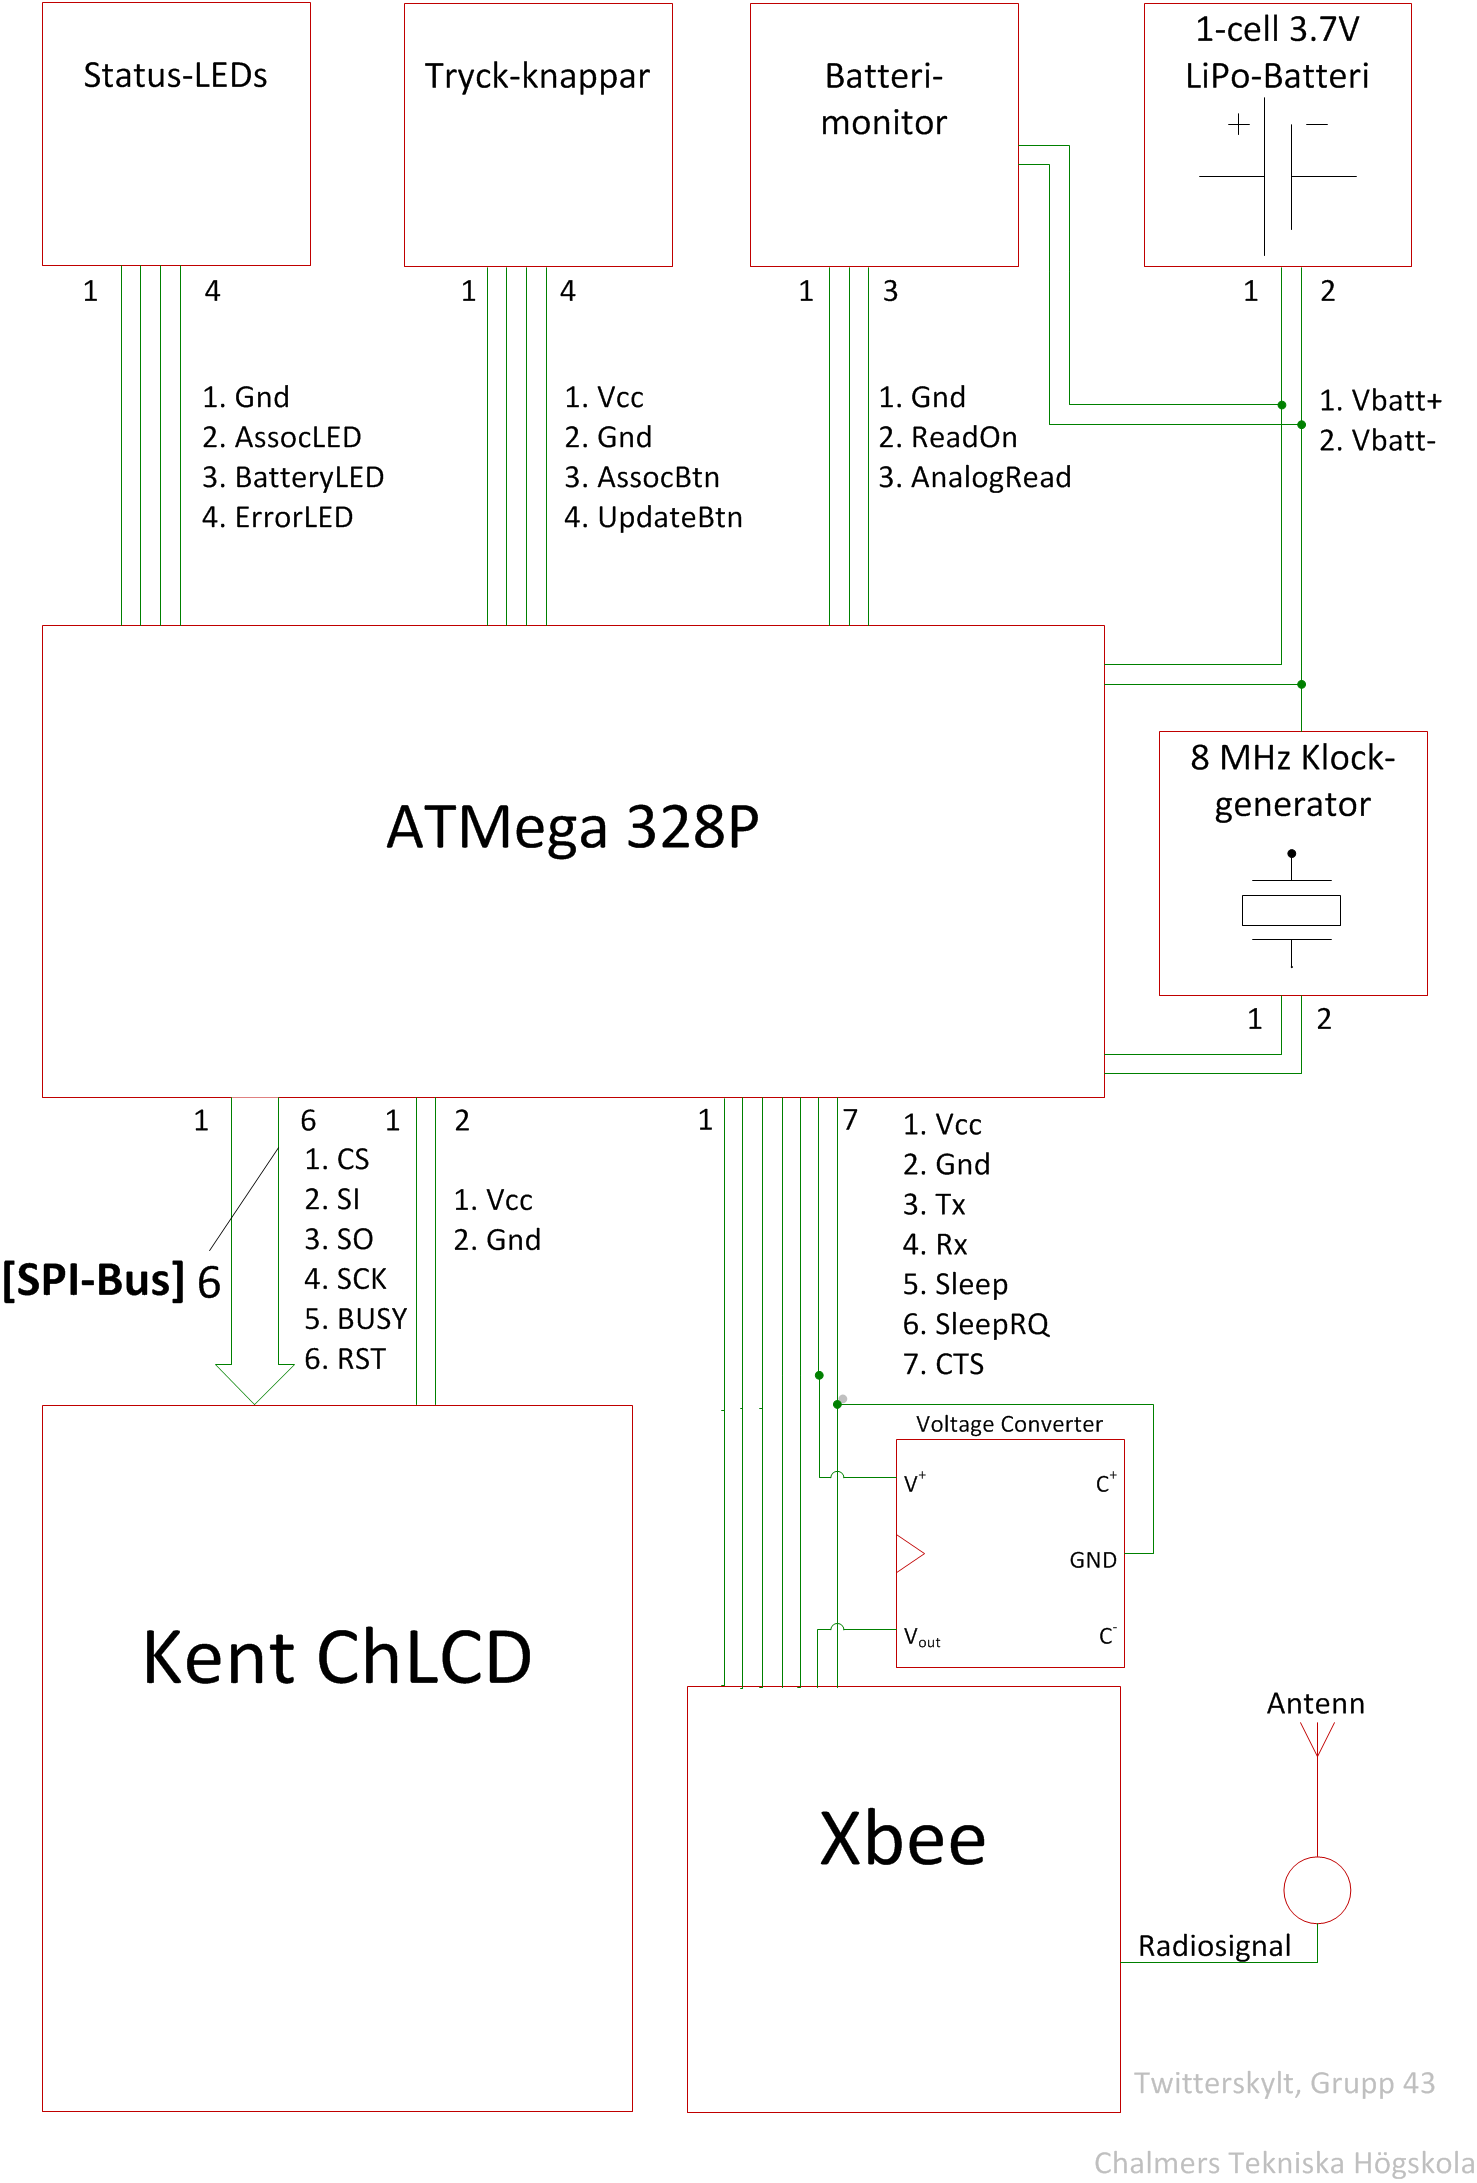
\includegraphics[scale=0.6, angle=0]{block_skylt.png}
\label{fig:block_skylt}
\caption{Blockschema, skylt}
\end{figure}
\pagebreak

\section{Kopplingsschema för stödkretsar i basstation}

\begin{figure}[H]
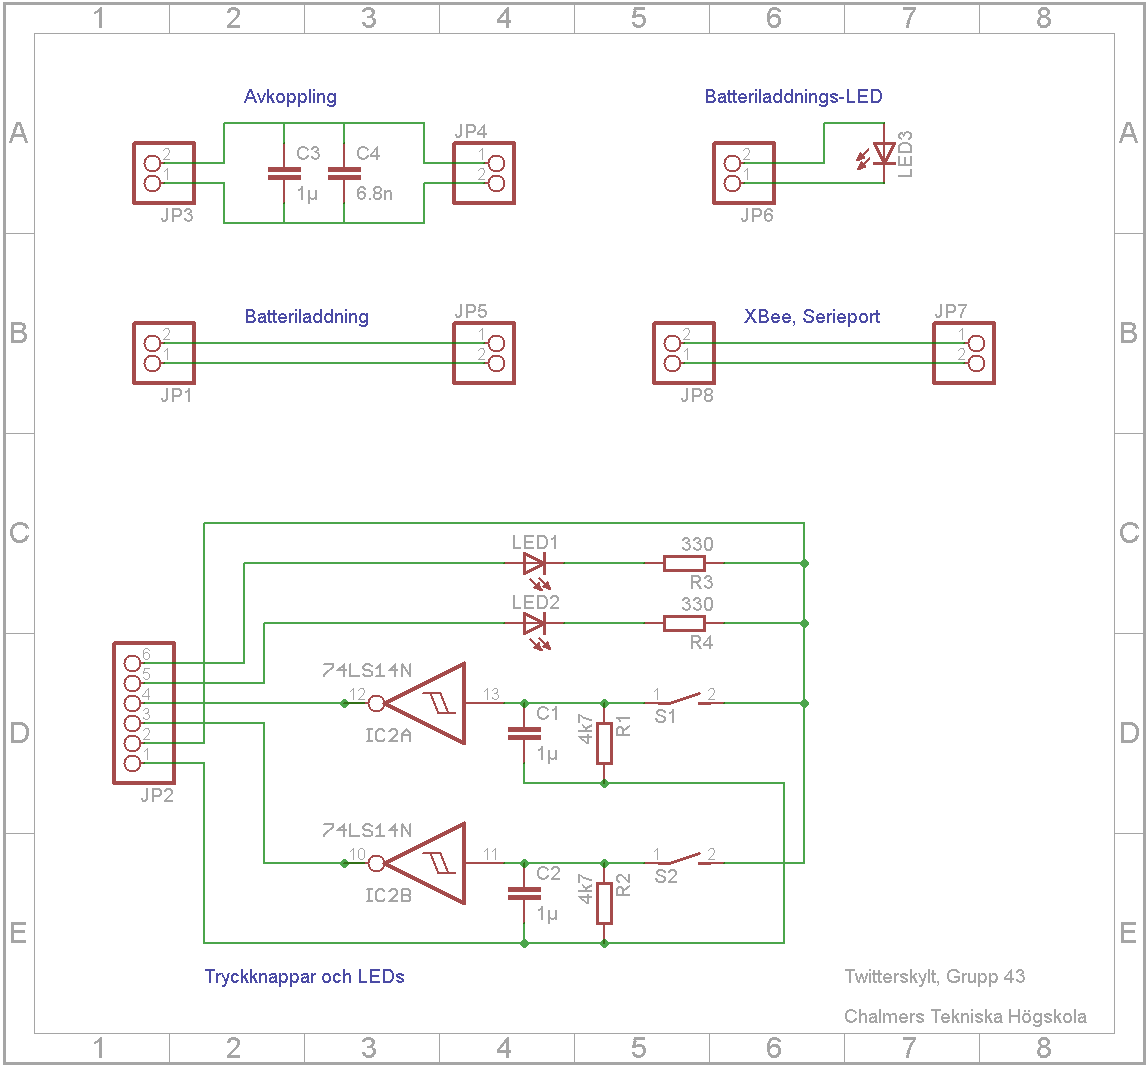
\includegraphics[scale=1.0, angle=0]{sch_bas.png}
\label{fig:block_skylt}
\caption{Kopplingsschema, bas}
\end{figure}
\pagebreak

\section{Kopplingsschema för stödkretsar i skyltmodul}

\begin{figure}[H]
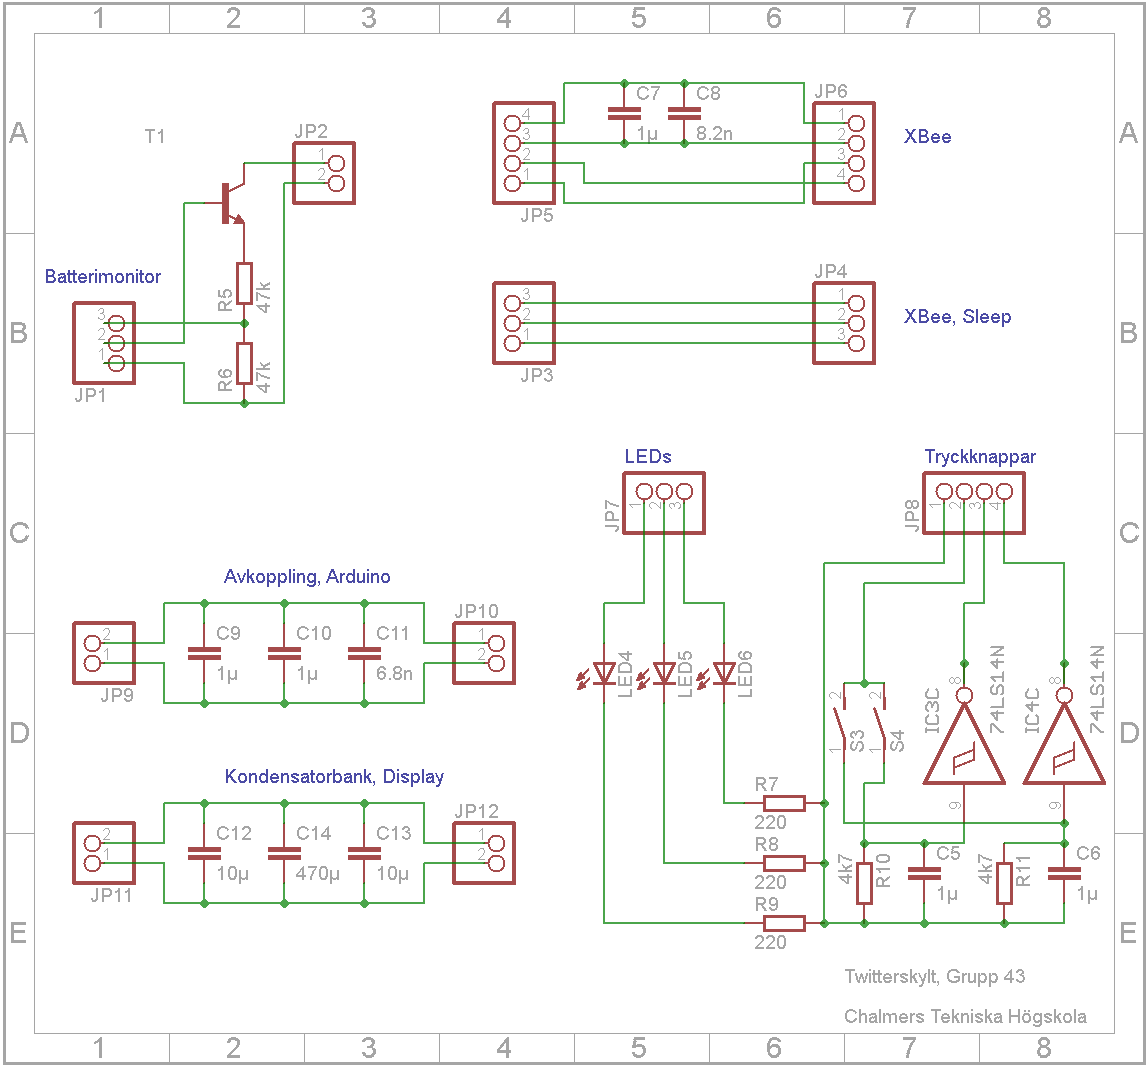
\includegraphics[scale=1.0, angle=0]{sch_skylt.png}
\label{fig:block_skylt}
\caption{Kopplingsschema, skylt}
\end{figure}
\pagebreak

\section{Komponentlista, stödkretsar}

\begin{table}[h]
\centering
	\begin{tabular}{|l|c|r|}
	{\bf Namn} & {\bf Värde} & {\bf Typ} \\
	C1-C3			& 1$\mu$	& Kapacitans \\
	C4			& 6.8n		& Kapactians \\		
	C5-C7			& 1$\mu$	& Kapacitans \\
	C8			& 8.2n		& Kapaictans \\
	C9-C10			& 1$\mu$	& Kapactians \\
	C11			& 6.8n		& Kapacitans \\
	C12-C13			& 10$\mu$	& Kapactians \\
	C14			& 470$\mu$	& Kapactians \\
	IC1			& -		& 7414-Schmitt \\
	IC2			& -		& TMP36 \\
	IC3-IC4			& -		& 7414-Schmitt \\
	LED1-LED3		& -		& LED (5mm) \\
	LED4-LED6		& -		& LED (3mm) \\
	R1-R2			& 4k7		& Resistans \\
	R3-R4			& 330		& Resistans \\
	R5-R6			& 47k		& Resistans \\
	R7-R9			& 220		& Resistans \\
	R10-R11			& 4k7		& Resistans \\
	S1-S4			& -		& Tryckknapp \\
	T1                      & -		& 2N4124-NPN-TO92-CBE \\
	\end{tabular}
\caption{Komponentlista, stödkretsar}
\label{tab:komponenttable}
\end{table}
\pagebreak

\section{Komponentlista, huvudsystem}

\begin{table}[h]
\centering
	\begin{tabular}{|l|r|}
	{\bf Komponent/Kort} & {\bf Tillverkare} \\
	Arduino Mega 2560                  & Arduino \\
	Arduino Ethernet Shield            & Arduino \\
	XBee Shield                        & Arduino \\
	XBee Series 1 Whip Antenna 1mW     & Digi International \\
	USB LiPoly Charger Single Cell     & Sparkfun Electronics Inc. \\
	\end{tabular}
\caption{Komponentlista, basstation}
\label{tab:korttable_bas}
\end{table}

\begin{table}[h]
\centering
	\begin{tabular}{|l|r|}
	{\bf Komponent/Kort} & {\bf Tillverkare} \\
	Arduino Mega 2560                  & Arduino \\
	Arduino Ethernet Shield            & Arduino \\
	XBee Shield                        & Arduino \\
	XBee Series 1 Whip Antenna 1mW     & Digi International \\
	USB LiPoly Charger Single Cell     & Sparkfun Electronics Inc. \\
	\end{tabular}
\caption{Komponentlista, skylt}
\label{tab:korttable_skylt}
\end{table}
\pagebreak

\section{Arbetsfördelning}
Nedan redovisas de gruppmedlemmar som varit huvudansvariga för de olika områdena under projektet. Till viss del överlappar områden, och gruppmedlemmar har varit inblandade i andra områden än de som står listade nedan.\\

{\bf Konstruktion}
	\begin{enumerate}
    	\item Tweethämtning - {\it Kim}
    	\item Parsing - {\it Jakob}
    	\item Formattering - {\it Kim, Jakob}
    	\item Användarkonfigurering (SD-kort) - {\it Andreas, Anton}
    	\item Ethernet - {\it Andreas, Anton}
    	\item Radiolänk - {\it Lars, Fredrik}
    	\item Display - {\it Lars, Anton}
    	\item Övrig elektronik och mekanik - {\it Fredrik}\\
    	\end{enumerate}
{\bf Rapport}
	\begin{enumerate}
    	\item Inledning
    	\item Bakomliggande tekniker och tjänster
    	\item Arbetsmetod
    	\item Systembeskrivning
    	\item Resultat
    	\item Diskussion och slutsatser
    	\item Appendix
	\end{enumerate}
{\bf Presentation}
	\begin{enumerate}
 	\item Halvtidsredovisning - Kim, Andreas
    	\item Slutpresentation
    	\item Opponering
    	\item Utställningsaffisch - Jakob\\
	\end{enumerate}
		
\end{document}
